\documentclass[times, utf8, zavrsni]{fer}
\usepackage{booktabs}

\usepackage[croatian]{babel} 
\usepackage{amssymb}
\usepackage{amsmath}
\usepackage{txfonts}
\usepackage{mathdots}
\usepackage{titlesec}
\usepackage{array}
\usepackage{lastpage}
\usepackage{etoolbox}
\usepackage{tabularray}
\usepackage{color, colortbl}
\usepackage{adjustbox}
\usepackage{geometry}
\usepackage[classicReIm]{kpfonts}
\usepackage{hyperref}
\usepackage{fancyhdr}

\usepackage{float}
\usepackage{setspace}
\restylefloat{table}


\linespread{1.3} %razmak između redaka

\geometry{a4paper, left=1in, top=1in,}  %oblik stranice

\hypersetup{ colorlinks, citecolor=black, filecolor=black, linkcolor=black,	urlcolor=black }   %izgled poveznice

%boja za privatni i udaljeni kljuc u tablicama
\definecolor{LightBlue}{rgb}{0.9,0.9,1}
\definecolor{LightGreen}{rgb}{0.9,1,0.9}

%Promjena teksta za dugačke tablice
\DefTblrTemplate{contfoot-text}{normal}{Nastavljeno na idućoj stranici}
\SetTblrTemplate{contfoot-text}{normal}
\DefTblrTemplate{conthead-text}{normal}{(Nastavljeno)}
\SetTblrTemplate{conthead-text}{normal}
\DefTblrTemplate{middlehead,lasthead}{normal}{Nastavljeno od prethodne stranice}
\SetTblrTemplate{middlehead,lasthead}{normal}

\newenvironment{packed_enum}{
	\begin{enumerate}
		\setlength{\itemsep}{0pt}
		\setlength{\parskip}{0pt}
		\setlength{\parsep}{0pt}
	}{\end{enumerate}}
	
\newenvironment{packed_item}{
	\begin{itemize}
		\setlength{\itemsep}{0pt}
		\setlength{\parskip}{0pt}
		\setlength{\parsep}{0pt}
	}{\end{itemize}}

\begin{document}

% Ispis stranice s napomenom o umetanju izvornika rada. Uklonite naredbu \izvornik ako želite izbaciti tu stranicu.
% \izvornik

% Dodavanje zahvale ili prazne stranice. Ako ne želite dodati zahvalu, naredbu ostavite radi prazne stranice.
\zahvala{}

\tableofcontents

\chapter{Uvod}
    U okviru završnog rada potrebno je izgraditi mobilnu aplikaciju \textit{Pole Flow App} za podršku aktivnostima plesnog kluba. Aplikacija će služiti lakšoj organizaciji treninga i članova kluba. Cilj aplikacije je automatizirati poslovne procese kluba s naglaskom na organizaciju upisa i aktivnosti koje se trenutno obavljaju slanjem poruka između članova i voditelja. 
    
    Trenutna organizacija je na \textit{WhatsApp} grupama i u bilježnicama trenera. Svaka grupa u klubu se sastoji od 4-6 članova te ima određeni termin treninga, vrstu aktivnosti i svoju \textit{WhatsApp} grupu. U \textit{WhatsApp} grupi se obavljaju dogovori među članovima, šalju se obavijesti vezane za klub od strane trenera te članovi javljaju o svom ne/dolasku na određeni trening. Članovi biraju sami u kojim aktivnostima žele sudjelovati, po dogovoru se sastavljaju nove grupe te odabire termin održavanja treninga na tjednoj bazi. Članovi kluba mogu sudjelovati u različitim aktivnostima u plesnom klubu: Pole Flow, Pole Flow Dupli, Exotic Flow i Fleksibilnost. Treninzi se održavaju od ponedjeljka do petka, a po potrebi i vikendom. 
    
    Trenutna situacija u plesnom klubu je takva da se prije treninga ne zna o dolaznosti članove određene grupe te se događa da trener čeka članove koji se uopće neće pojaviti. Izgubljeno vrijeme se moglo puno bolje iskoristiti, samo da se znala situacija među članovima. Drugi primjer situacije je da u slučaju nedolaska nekolicine, slobodna mjesta u terminu bi se mogla popuniti s članovima drugih grupa koje bih trebale nadoknaditi neodrađene treninge. 
    
    Kako bi se izbjegli budući nesporazumi, nedostaci, izgubljeno vrijeme i resursi, riješenje želimo postići mobilnom aplikacijom kojoj bi mogli pristupiti svi korisnici u plesnom klubu. Mobilna-aplikacija različitim korisnicima omogućuje:
    Registraciju i prijavu na sustav kao član kluba, Registraciju i prijavu na sustav kao trener, Prijavu na sustav kao administrator, Pregled raspored treninga, Pregled obavijesti, Pregled galerije, Pregled korisničkog profila, Kreiranje i uređivanje grupa,te Uređivanje stanja članarina.
	
	
	
        \pagebreak
        
\chapter{Korištene tehnologije i alati}
		
			 Za izradu dijagrama baze podataka korišten je alat \textit{dbdiagram}\footnote{\url{https://dbdiagram.io/}}, a kao sustav za upravljanjem izvornim kodom \textit{Git}\footnote{\url{https://git-scm.com/}}. Udaljeni repozitoriji projekta dostupan je na web platformi \textit{GitLab}\footnote{\url{https://gitlab.com/}}.
			 
			Za izradu aplikacije korišten je uređivač koda \textit{Visual Studio Code\footnote{\url{https://code.visualstudio.com/}}} tvrke Microsoft. VSC je uređivač koda dostupan na  \textit{Windowsu},  \textit{Linuxu} i  \textit{macOS-u} i podržava uređivanje koda većine popularnih programskih jezika putem ekstenzija, a posebno je prigodan za razvoj web i mobilnih aplikacija zato što ima ugrađenu potporu za JavaScript, TypeScript, CSS, JSON i HTML. VSC-ov izvorni kod se nalazi na  \textit{GitHub-u}\footnote{\url{https://github.com/microsoft/vscode}}.
			 
			 
			 Aplikacija je napisana koristeći programski jezik \textit{JavaScript}\footnote{\url{https://www.javascript.com/}} i \textit{Node.js}\footnote{\url{https://nodejs.org/en/}}. Za frontend je uz to korišten alat \textit{React Native}\footnote{\url{https://reactnative.dev/}}, a za backend je korišten programski okvir \textit{Express}\footnote{\url{https://expressjs.com/}}. \textit{React Native}, takoder
            poznat kao React.js ili ReactJS, je biblioteka u JavaScriptu za izgradnju korisničkih sučelja. React se najčešće koristi kao osnova u razvoju web ili mobilnih aplikacija. Složene aplikacije u Reactu obično zahtijevaju korištenje dodatnih biblioteka za interakciju s API-jem. \textit{Node.js} je okruženje koje izvodi JavaScript kod izvan web browsera i dopušta stvaranje dinamičnih web aplikacija.  Express jedan od najpopularnijih Node.js radnih okvira za programiranje serverske strane web aplikacija
			 
			 
			 Također korišten je alat \textit{PostgresSQL}\footnote{\url{https://www.postgresql.org/}} za upravljanje bazom podataka.
			
			
			\pagebreak 

\chapter{Opis programske podrške za plesni klub}    
    \section{Korisnici sustava}
    
		Tipovi korisnika na platformi \textit{Pole Flow App} su neregistrirani, članovi kluba, treneri i administratori. Opis mogućnosti tih različitih tipova korisnika, tim redom su opisani u nastavku.
		
		\subsection{Neregistrirani korisnici}
		Pri učlanjenju u plesni klub, neregistrirani korisnik dobiva pristup aplikaciji te mu je omogućena registracija u sustav i kreiranje novog korisničkog računa. Za kreiranje novo računa potrebni su sljedeći podaci:
		 \begin{packed_item}
		    \item Ime korisnika
		    \item Prezime korisnika
		    \item E-mail adresa
		    \item Broj mobitela
		    \item Datum rođenja
		    \item Lozinka
		    \item Uloga (član kluba ili trener)
	    \end{packed_item}
	
	    Neregistrirani korisnik zatim odabire termine koji bi mu odgovarali za buduće treninge. Ta informacija je vrlo korisna administratoru pri stvaranju grupa i odabira idealnog termina koji odgovara svim članovima grupe.
		
		
		\subsection{Članovi kluba}
		Nakon registracije članovi kluba imaju mogućnost pregleda informacija o plesnom klubu, treninzima te svojim podacima.  
		
		\\Članovi kluba se prijavljuju u sustav s e-mail adresom i lozinkom. Korisničke podatke je moguće pregledati te izmijeniti na korisničkom profilu. Uz podatke koji su uneseni pri prijavi moguć je pregled stanja i iznosa članarine te godine treniranje tj. iskustva u klubu. U slučaju promjene podataka omogućeno je uređivanje korisničkog računa. 
		
		\\Kako bi pratili novosti i promjene vezane za plesni klub, članovi kluba imaju mogućnost pregleda obavijesti na početnoj stranici. Na početnoj stranici se također zna nalaziti podsjetnik za trening koji se planira održati tog dana. Putem podsjetnika član kluba može dati povratnu informaciju treneru i administratoru o svom dolasku ili ne dolasku na određeni trening. 
		
		\\Član kluba osim  pregleda današnjeg trening, može pregledati raspored treninga po datumima. Raspored treninga prikazuje sve treninge koji se održavaju za grupu kojoj član kluba pripada. 
		
		\\Uz sve navedeno, ima mogućnost pregleda galerije u kojoj se nalaze fotografije koje je administrator objavio s treninga, profesionalnog slika, itd. 
		
		\subsection{Treneri}
		Nakon registracije treneri imaju mogućnost jednake članovima kluba. Treneri mogu istovremeno biti trener jednoj grupi i trenirati kao član kluba u drugoj.
		
		\\Treneri također imaju mogućnost pregleda raspored treninga po datumima. Raspored treninga prikazuje sve treninge koji se održavaju za grupu kojoj trener pripada te sve treninge grupa koje trenira. Za sve treninge koji su održani može dati povratnu informaciju o dolascima članova na trening.
	
		\subsection{Administrator}
		Administratoru je dostupa pregled svih informacija i podataka na aplikaciji. Ima mogućnosti dodavanja, uređivanja i brisanja podataka.
		
		\\Dostupan mu je pregled novo registriranih kao i općenito svih korisnika. Omogućen mu je pregled i podataka o korisnicima kao što su ime, prezime, iskustvo i članarina. Administrator u trenutku kada mu Član kluba ili Trener plati članarinu, može označiti na njihovom korisničkom računu da je članarina plaćena za određen mjesec. U slučaju ispisa članova iz kluba ili otkaza trenera, samo administrator ima mogućnost brisanja korisničkih profila iz sustava.
		
		\\Administrator po dogovoru s grupom stvara grupu u sustavu te joj pridjeljuje termin treninga koji odgovara svim članovima grupe i treneru. On grupu kasnije može uređivati te po potrebi i obrisati.
		
		\\Za pisanje, uređivanje i brisanje obavijesti na početnoj stranici je zadužen administrator kao i za dodavanje, uređivanje i brisanje fotografija u galeriji.
		
		\\U pregledu rasporeda su mu prikazani treninzi svih grupa.
		
		\pagebreak
		
		\section{Funkcionalni zahtjevi}		
			
			\noindent \textbf{Dionici:}
			
			\begin{packed_enum}
				
				\item Član Kluba
				\item Trener				
				\item Administrator
				\item Razvojni tim
				
			\end{packed_enum}
			
			\noindent \textbf{Aktori i njihovi funkcionalni zahtjevi:}
			
			
			\begin{packed_enum}
				\item  \underbar{Neregistrirani korisnik (inicijator) može:}
				
				\begin{packed_enum}
					
					\item registrirati se i otvoriti račun na platformi
					
				\end{packed_enum}
			
				\item  \underbar{Registrirani Član Kluba može:}
				
				\begin{packed_enum}
					
					\item pregledavati obavijesti
					\item pregledavati galeriju
					\item pregledavati i uređivati osobne podatke
					\item pregledavati raspored treninga za grupe u kojima trenira
					\item pregledavati stanje članarine
					\item dati povratnu informaciju o ne/dolasku na trening
					\item prijaviti se u sustav
					
				\end{packed_enum}
			
				\item  \underbar{Trener (inicijator) može:}
				
				\begin{packed_enum}
					
					\item pregledavati obavijesti
					\item pregledavati galeriju
					\item pregledavati i uređivati osobne podatke
					\item pregledavati raspored trening za grupa koje trenira
					\item dati povratnu informaciju o dolaznosti na trening
					\item pregledavati stanje članarine
					\item prijaviti se u sustav
					
				\end{packed_enum}
			
				\item  \underbar{Administrator (inicijator) može:}
				
				\begin{packed_enum}
					
					\item pregledavati obavijesti
					\item pisanje, uređivanje i brisanje obavijesti
					\item pregledavati galeriju
				    \item pisanje, uređivanje i brisanje fotografija u galeriji
					\item pregledavati i uređivati osobne podatke
					\item pregledavati novo registrirane korisnike
					\item pregledavati korisnike
					\item pregledavati grupe
					\item stvaranje, uređivanje i brisanje grupa
					\item pregledavati osobne podatke o korisnicima
					\item pregledavati i uređivati stanja članarine korisnika
					\item pregledavati raspored trening za sve grupe
					\item prijaviti se u sustav
					
				\end{packed_enum}
			
				\item  \underbar{Baza podataka (sudionik):}
				
				\begin{packed_enum}
					
					\item pohranjuje podatke o svim korisnicima platforme
					\item pohranjuje podatke o svim grupama koje su na platformi
					\item pohranjuje podatke o svim treninzima koje su na platformi
					\item pohranjuje dodatne sadržaje poput obavijesti i fotografija
					
				\end{packed_enum}
				
			\end{packed_enum}
			
			\eject 
			
				
			\subsection{Obrasci uporabe}
			\noindent \underbar{\textbf{UC1 - Registracija novog korisnika}}
					\begin{packed_item}
						
						\item \textbf{Glavni sudionik: } Korisnik
						\item  \textbf{Cilj:} Dobiti pristup aplikaciji
						\item  \textbf{Sudionici:} Baza podataka
						\item  \textbf{Preduvjet:} Korisnik se odlučio učlaniti u klub
						\item  \textbf{Opis osnovnog tijeka događaja:}
						
						\item[] \begin{packed_enum}
							
							\item Korisnik odabire opciju za registraciju
							\item Korisnik unosi potrebne podatke za kreiranje korisničkog računa u sustavu
							\item Potvrda o validaciji unesenih podataka
							\item Potvrda o ispravnosti unesenih podataka
							\item Korisnik odabire termine koji mu odgovaraju za treningu
							\item Pristup korisničkim funkcijama

							
						\end{packed_enum}
						
						\item  \textbf{Opis mogućih odstupanja:}
						
						\item[] \begin{packed_item}
							
							\item[2.a] Pružanje neispravnog podatka
							\item[] \begin{packed_enum}
								
								\item Aplikacija obavještava korisnika o neuspješnom upisu s obzirom na validaciju podataka
								\item Aplikacija obavještava korisnika o neuspješnom upisu s obzirom na bazu sustava
								\item Korisnik mijenja unesene podatke ili odustaje od registracije
								
							\end{packed_enum}
							
						\end{packed_item}
					\end{packed_item}
		    \noindent \underbar{\textbf{UC2 - Prijava korisnika}}
					\begin{packed_item}
						
						\item \textbf{Glavni sudionik: } Korisnik
						\item  \textbf{Cilj:} Dobiti pristup aplikaciji
						\item  \textbf{Sudionici:} Baza podataka
						\item  \textbf{Preduvjet:} Korisnik je registriran i postoji u bazi podataka
						\item  \textbf{Opis osnovnog tijeka događaja:}
						
						\item[] \begin{packed_enum}
							
							\item Korisnik odabire opciju za prijavu
							\item Korisnik unosi e-mail adresu i lozinku
							\item Potvrda o ispravnosti unesenih podataka
							\item Pristup korisničkim funkcijama
							
						\end{packed_enum}
						
						\item  \textbf{Opis mogućih odstupanja:}
						
						\item[] \begin{packed_item}
							
							\item[2.a] Pružanje neispravnog podatka
							\item[] \begin{packed_enum}
								
								\item Aplikacija obavještava korisnika o neuspješnom upisu
								\item Korisnik mijenja unesene podatke ili odustaje od prijave
								
							\end{packed_enum}
							
						\end{packed_item}
					\end{packed_item}
					
		    \noindent \underbar{\textbf{UC3 - Pregled korisničkog računa}}
					\begin{packed_item}
						
						\item \textbf{Glavni sudionik: } Korisnik
						\item  \textbf{Cilj:} Pregled korisničkih podataka
						\item  \textbf{Sudionici:} Baza podataka
						\item  \textbf{Preduvjet:} Prijava
						\item  \textbf{Opis osnovnog tijeka događaja:}
						
						\item[] \begin{packed_enum}
							
							\item Korisnik otvara stranicu s korisničkim računom
							\item Prikaz osobnih podataka korisnika
							
						\end{packed_enum}
						
					\end{packed_item}
					
			\noindent \underbar{\textbf{UC4 - Uređivanje korisničkog računa}}
					\begin{packed_item}
						
						\item \textbf{Glavni sudionik: } Korisnik
						\item  \textbf{Cilj:} Promijeniti osobne podatke korisnika
						\item  \textbf{Sudionici:} Baza podataka
						\item  \textbf{Preduvjet:} Prijava
						\item  \textbf{Opis osnovnog tijeka događaja:}
						
						\item[] \begin{packed_enum}
							
							\item Korisnik otvara stranicu s korisničkim računom
							\item Korisnik odabire opciju promjene osobnih podataka
							\item Korisnik mijenja podatke svog korisničkog računa
							\item Korisnik sprema promjene
							\item Baza podataka se ažurira
							
						\end{packed_enum}
						
					\end{packed_item}
					
			\noindent \underbar{\textbf{UC5 - Pregled članarine}}
					\begin{packed_item}
						
						\item \textbf{Glavni sudionik: } Član Kluba
						\item  \textbf{Cilj:} Pregled članarine
						\item  \textbf{Sudionici:} Baza podataka
						\item  \textbf{Preduvjet:} Prijava
						\item  \textbf{Opis osnovnog tijeka događaja:}
						
						\item[] \begin{packed_enum}
							
							\item Korisnik odabire opciju pregleda korisničkog računa
							\item Pregled iznosa i statusa članarine za trenutni mjesec
							
						\end{packed_enum}
						
					\end{packed_item}
					
			\noindent \underbar{\textbf{UC6 - Pregled nadoknada}}
					\begin{packed_item}
						
						\item \textbf{Glavni sudionik: } Član Kluba
						\item  \textbf{Cilj:} Pregled broja nadoknada
						\item  \textbf{Sudionici:} Baza podataka
						\item  \textbf{Preduvjet:} Prijava
						\item  \textbf{Opis osnovnog tijeka događaja:}
						
						\item[] \begin{packed_enum}
							
							\item Korisnik odabire opciju pregleda korisničkog računa
							\item Pregled broja nadoknada
							
						\end{packed_enum}
						
					\end{packed_item}
					
			\noindent \underbar{\textbf{UC7 - Pregled galerije}}
					\begin{packed_item}
						
						\item \textbf{Glavni sudionik: } Korisnik
						\item  \textbf{Cilj:} Pregled fotografija
						\item  \textbf{Sudionici:} Baza podataka
						\item  \textbf{Preduvjet:} Prijava
						\item  \textbf{Opis osnovnog tijeka događaja:}
						
						\item[] \begin{packed_enum}
							
							\item Korisnik odabire opciju pregleda galerije
							\item Korisnik odabire fotografiju
							\item Prikaz fotografiju u punoj veličini
							
						\end{packed_enum}
						
					\end{packed_item}
					
			\noindent \underbar{\textbf{UC8 - Dodavanje fotografije u galeriju}}
					\begin{packed_item}
						
						\item \textbf{Glavni sudionik: } Administrator
						\item  \textbf{Cilj:} Dodavanje fotografije u galeriju
						\item  \textbf{Sudionici:} Baza podataka
						\item  \textbf{Preduvjet:} Administrator je prijavljen
						\item  \textbf{Opis osnovnog tijeka događaja:}
						
						\item[] \begin{packed_enum}
							
							\item Administrator odabire opciju pregleda galerije
							\item Administrator odabire opciju dodavanja nove fotografije
							\item Administrator odabire fotografiju sa svog mobilnog uređaja
							\item Unos fotografije u bazu podataka
							\item Preusmjeravanje na prikaz galerije
							
							
						\end{packed_enum}
						
					\end{packed_item}
			
			\noindent \underbar{\textbf{UC9 - Brisanje fotografije iz galerije}}
					\begin{packed_item}
						
						\item \textbf{Glavni sudionik: } Administrator
						\item  \textbf{Cilj:} Brisanje fotografije iz galerije
						\item  \textbf{Sudionici:} Baza podataka
						\item  \textbf{Preduvjet:} 
						\item[] \begin{packed_enum}
							
							\item Administrator je prijavljen
							\item Odabrana fotografija postoji u bazi podataka
							
						\end{packed_enum}
						
						\item  \textbf{Opis osnovnog tijeka događaja:}
						
						\item[] \begin{packed_enum}
							
							\item Administrator odabire opciju pregleda galerije
							\item Administrator odabire fotografiju koju želi obrisati
							\item Brisanje fotografije iz baze podatka
							\item Preusmjeravanje na prikaz galerije
							
						\end{packed_enum}
						
					\end{packed_item}
					
			\noindent \underbar{\textbf{UC10 - Pregled rasporeda svih treninga}}
					\begin{packed_item}
						
						\item \textbf{Glavni sudionik: } Administrator
						\item  \textbf{Cilj:} Pregled rasporeda svih treninga
						\item  \textbf{Sudionici:} Baza podataka
						\item  \textbf{Preduvjet:} Administrator je prijavljen
						\item  \textbf{Opis osnovnog tijeka događaja:}
						
						\item[] \begin{packed_enum}
							
							\item Administrator odabire opciju pregleda rasporeda treninga
							\item Prikaz svih treninga po datumima
							
							
						\end{packed_enum}
						
					\end{packed_item}
					
			\noindent \underbar{\textbf{UC11 - Pregled rasporeda određenih treninga}}
					\begin{packed_item}
						
						\item \textbf{Glavni sudionik: } Korisnik
						\item  \textbf{Cilj:} Pregled rasporeda treninga
						\item  \textbf{Sudionici:} Baza podataka
						\item  \textbf{Preduvjet:} Korisnik je prijavljen
						\item  \textbf{Opis osnovnog tijeka događaja:}
						
						\item[] \begin{packed_enum}
							
							\item Korisnik odabire opciju pregleda rasporeda treninga
							\item Prikaz treninga po datumima
							    \item[] \begin{packed_enum}
							
        							\item Ako je korisnik Član kluba onda mu se prikazuju treninzi grupa koji je član
        							\item Ako je korisnik Trener onda mu se prikazuju treninzi grupa koje trenira
        							
        							
        						\end{packed_enum}
							
							
						\end{packed_enum}
						
					\end{packed_item}
			
			\noindent \underbar{\textbf{UC12 - Pregled obavijesti}}
					\begin{packed_item}
						
						\item \textbf{Glavni sudionik: } Korisnik
						\item  \textbf{Cilj:} Pregled obavijesti
						\item  \textbf{Sudionici:} Baza podataka
						\item  \textbf{Preduvjet:} Korisnik je prijavljen
						\item  \textbf{Opis osnovnog tijeka događaja:}
						
						\item[] \begin{packed_enum}
							
							\item Prikaz obavijesti na početnoj stranici
							
							
						\end{packed_enum}
						
					\end{packed_item}
					
			\noindent \underbar{\textbf{UC13 - Podsjetnik na trening}}
					\begin{packed_item}
						
						\item \textbf{Glavni sudionik: } Član Kluba
						\item  \textbf{Cilj:} Korisnik daje povratnu informaciju treneru o ne/dolasku na trening tog dana
						\item  \textbf{Sudionici:} Trener, Baza podataka
						\item  \textbf{Preduvjet:} Član Kluba je prijavljen
						\item  \textbf{Opis osnovnog tijeka događaja:}
						
						\item[] \begin{packed_enum}
							
							\item Korisnik se prikazuje na glavnoj stranici opcija kvačice („Dolazim“) i križića („Ne dolazim“) za nadolazeći trening
							\item Korisnik odabire jednu od opcija prije isteka vremena 
							
							
						\end{packed_enum}
						
						\item  \textbf{Opis mogućih odstupanja:}
						
						\item[] \begin{packed_enum}
							
							\item U slučaju ne odabira niti jedne opcije prije isteka vremena, korisniku se u raspored dodaju termini nadoknade treninga
							
						\end{packed_enum}
						
					\end{packed_item}
					
			\noindent \underbar{\textbf{UC14 - Informacije o nadolazećem treningu}}
					\begin{packed_item}
						
						\item \textbf{Glavni sudionik: } Korisnik
						\item  \textbf{Cilj:} Korisnik dobiva informacije o nadolazećem treningu
						\item  \textbf{Sudionici:} Baza podataka
						\item  \textbf{Preduvjet:} 
						
						\item[] \begin{packed_enum}
							
							\item Korisnik je prijavljen
							\item Odabrani trening nije obavljen
							
							
						\end{packed_enum}
						
						\item  \textbf{Opis osnovnog tijeka događaja:}
						
						\item[] \begin{packed_enum}
							
							\item Korisnik odabire opciju pregleda rasporeda treninga
							\item Korisnik odabire trening koji nije obavljen
							\item Korisnik dobiva informacije o treningu
							
							
						\end{packed_enum}
						
					\end{packed_item}
					
		    \noindent \underbar{\textbf{UC15 - Povratna informacija o dolaznosti na trening}}
					\begin{packed_item}
						
						\item \textbf{Glavni sudionik: } Trener
						\item  \textbf{Cilj:} Trener daje povratnu informaciju dolaznosti na trening
						\item  \textbf{Sudionici:} Baza podataka
						\item  \textbf{Preduvjet:} 
						
						\item[] \begin{packed_enum}
							
							\item Trener je prijavljen
							\item Odabrani trening je obavljen
							
							
						\end{packed_enum}
						
						\item  \textbf{Opis osnovnog tijeka događaja:}
						
						\item[] \begin{packed_enum}
							
							\item Trener odabire opciju pregleda rasporeda treninga
							\item Trener odabire trening koji je obavljen
							\item Trener dobiva informacije o treningu
							\item Trener odabire koji članovi kluba su došli ili nisu došli na trening
							\item Trener pohranjuje informacije u bazu podataka
							\item Preusmjeravanje na pregled rasporeda treninga
							
							
						\end{packed_enum}
						
					\end{packed_item}
					
			\noindent \underbar{\textbf{UC16 - Pregled svih grupa}}
					\begin{packed_item}
						
						\item \textbf{Glavni sudionik: } Administrator
						\item  \textbf{Cilj:} Pregled svih grupa
						\item  \textbf{Sudionici:} Baza podataka
						\item  \textbf{Preduvjet:} Administrator je prijavljen
						\item  \textbf{Opis osnovnog tijeka događaja:}
						
						\item[] \begin{packed_enum}
							
							\item Administrator odabire opciju pregleda grupa
							\item Prikaz svih grupa s opcijom pretraživanja po imenu grupe
							
							
						\end{packed_enum}
						
					\end{packed_item}
					
			\noindent \underbar{\textbf{UC17 - Pregled detalja grupe}}
					\begin{packed_item}
						
						\item \textbf{Glavni sudionik: } Administrator
						\item  \textbf{Cilj:} Pregled detalja grupe
						\item  \textbf{Sudionici:} Baza podataka
						\item  \textbf{Preduvjet:} 
						
						\item[] \begin{packed_enum}
							
							\item Administrator je prijavljen
							\item Odabrana grupa postoji u bazi podataka
							
							
						\end{packed_enum}
						
						\item  \textbf{Opis osnovnog tijeka događaja:}
						
						\item[] \begin{packed_enum}
							
							\item Administrator odabire opciju pregleda grupa
							\item Prikaz svih grupa s opcijom pretraživanja po imenu grupe
							\item Administrator odabire grupu
							\item Prikaz informacija o grupi
							
							
						\end{packed_enum}
						
					\end{packed_item}
					
			\noindent \underbar{\textbf{UC18 - Izbacivanje članova kluba iz grupe}}
					\begin{packed_item}
						
						\item \textbf{Glavni sudionik: } Administrator
						\item  \textbf{Cilj:} Izbacivanje članova kluba iz grupe
						\item  \textbf{Sudionici:} Baza podataka
						\item  \textbf{Preduvjet:} 
						
						\item[] \begin{packed_enum}
							
							\item Administrator je prijavljen
							\item Odabrana grupa postoji u bazi podataka
							
							
						\end{packed_enum}
						
						\item  \textbf{Opis osnovnog tijeka događaja:}
						
						\item[] \begin{packed_enum}
							
							\item Administrator odabire opciju pregleda grupa
							\item Prikaz svih grupa s opcijom pretraživanja po imenu grupe
							\item Administrator odabire grupu
							\item Prikaz informacija o grupi
							\item Administrator klikom na člana kluba izbacuje ga iz grupe
							
							
						\end{packed_enum}
						
					\end{packed_item}
					
			\noindent \underbar{\textbf{UC19 - Uređivanje grupe}}
					\begin{packed_item}
						
						\item \textbf{Glavni sudionik: } Administrator
						\item  \textbf{Cilj:} Uređivanje grupe
						\item  \textbf{Sudionici:} Baza podataka
						\item  \textbf{Preduvjet:} 
						
						\item[] \begin{packed_enum}
							
							\item Administrator je prijavljen
							\item Odabrana grupa postoji u bazi podataka
							
							
						\end{packed_enum}
						
						\item  \textbf{Opis osnovnog tijeka događaja:}
						
						\item[] \begin{packed_enum}
							
							\item Administrator odabire opciju pregleda grupa
							\item Prikaz svih grupa s opcijom pretraživanja po imenu grupe
							\item Administrator odabire grupu
							\item Prikaz informacija o grupi
							\item Administrator klikom na "Uredi" odlazi na stranicu za uređivanje grupe
							\item Administrator uređuje grupe
							\item Kada završi s uređivanjem, novi podaci se pohranjuju u bazu
							\item Preusmjeravanje na pregled svih grupa
							
							
						\end{packed_enum}
						
					\end{packed_item}
					
			\noindent \underbar{\textbf{UC20 - Brisanje grupe}}
					\begin{packed_item}
						
						\item \textbf{Glavni sudionik: } Administrator
						\item  \textbf{Cilj:} Brisanje grupe
						\item  \textbf{Sudionici:} Baza podataka
						\item  \textbf{Preduvjet:} 
						
						\item[] \begin{packed_enum}
							
							\item Administrator je prijavljen
							\item Odabrana grupa postoji u bazi podataka
							
							
						\end{packed_enum}
						
						\item  \textbf{Opis osnovnog tijeka događaja:}
						
						\item[] \begin{packed_enum}
							
							\item Administrator odabire opciju pregleda grupa
							\item Prikaz svih grupa s opcijom pretraživanja po imenu grupe
							\item Administrator odabire grupu
							\item Prikaz informacija o grupi
							\item Administrator klikom na "Obriši" briše grupu iz baze
							\item Preusmjeravanje na pregled svih grupa
							
							
						\end{packed_enum}
						
					\end{packed_item}
					
			\noindent \underbar{\textbf{UC21 - Pregled korisnika}}
					\begin{packed_item}
						
						\item \textbf{Glavni sudionik: } Administrator
						\item  \textbf{Cilj:} Brisanje grupe
						\item  \textbf{Sudionici:} Baza podataka
						\item  \textbf{Preduvjet:} Administrator je prijavljen
						
						\item  \textbf{Opis osnovnog tijeka događaja:}
						
						\item[] \begin{packed_enum}
							
							\item Administrator odabire opciju pregleda korisnika
							\item Prikaz svih korisnika s opcijom pretraživanja po imenu i prezimenu korisnika
							
						\end{packed_enum}
						
					\end{packed_item}
					
			\noindent \underbar{\textbf{UC22 - Pregled detalja korisnika}}
					\begin{packed_item}
						
						\item \textbf{Glavni sudionik: } Administrator
						\item  \textbf{Cilj:} Pregled detalja korisnika
						\item  \textbf{Sudionici:} Baza podataka
						\item  \textbf{Preduvjet:} 
						
						\item[] \begin{packed_enum}
							
							\item Administrator je prijavljen
							\item Odabrani korisnik postoji u bazi podataka
							
							
						\end{packed_enum}
						
						\item  \textbf{Opis osnovnog tijeka događaja:}
						
						\item[] \begin{packed_enum}
							
							\item Administrator odabire opciju pregleda korisnika
							\item Prikaz svih korisnika s opcijom pretraživanja po imenu i prezimenu korisnika
							\item Administrator odabire korisnika
							\item Prikaz informacija o korisniku
							
							
						\end{packed_enum}
						
					\end{packed_item}
					
			\noindent \underbar{\textbf{UC23 - Uređivanje članarine korisnika}}
					\begin{packed_item}
						
						\item \textbf{Glavni sudionik: } Administrator
						\item  \textbf{Cilj:} Uređivanje članarine korisnika
						\item  \textbf{Sudionici:} Baza podataka
						\item  \textbf{Preduvjet:} 
						
						\item[] \begin{packed_enum}
							
							\item Administrator je prijavljen
							\item Odabrani korisnik postoji u bazi podataka
							
							
						\end{packed_enum}
						
						\item  \textbf{Opis osnovnog tijeka događaja:}
						
						\item[] \begin{packed_enum}
							
							\item Administrator odabire opciju pregleda korisnika
							\item Prikaz svih korisnika s opcijom pretraživanja po imenu i prezimenu korisnika
							\item Administrator odabire korisnika
							\item Prikaz statusa i iznosa članarina po mjesecu koje nisu plaćene
							\item Administrator klikom  na kvačicu, pohranjuje u bazu da je članarina plaćena
							
						\end{packed_enum}
						
						\item  \textbf{Opis mogućih odstupanja:}
						
						\item[] \begin{packed_enum}
							
							\item U slučaju da je korisnik platio sve članarine, stoji natpis "Sve članarine plaćene"
							
						\end{packed_enum}
						
					\end{packed_item}
					
			\noindent \underbar{\textbf{UC24 - Brisanje korisnika}}
					\begin{packed_item}
						
						\item \textbf{Glavni sudionik: } Administrator
						\item  \textbf{Cilj:} Brisanje korisnika
						\item  \textbf{Sudionici:} Baza podataka
						\item  \textbf{Preduvjet:} 
						
						\item[] \begin{packed_enum}
							
							\item Administrator je prijavljen
							\item Odabrani korisnik postoji u bazi podataka
							\item Odabrani korisnik se ispisuje iz kluba
							
							
						\end{packed_enum}
						
						\item  \textbf{Opis osnovnog tijeka događaja:}
						
						\item[] \begin{packed_enum}
							
							\item Administrator odabire opciju pregleda korisnika
							\item Prikaz svih korisnika s opcijom pretraživanja po imenu i prezimenu korisnika
							\item Administrator odabire korisnika
							\item Administrator klikom na "Obriši" briše korisnika iz baze
							\item Preusmjeravanje na pregled svih korisnika
							
						\end{packed_enum}
						
						
					\end{packed_item}
					
			\noindent \underbar{\textbf{UC25 - Stvaranje grupe}}
					\begin{packed_item}
						
						\item \textbf{Glavni sudionik: } Administrator
						\item  \textbf{Cilj:} Stvaranje grupe
						\item  \textbf{Sudionici:} Baza podataka
						\item  \textbf{Preduvjet:} 
						
						\item[] \begin{packed_enum}
							
							\item Administrator je prijavljen
							\item Administrator po dogovoru s grupa unosi podatke u sustav
							
							
						\end{packed_enum}
						
						\item  \textbf{Opis osnovnog tijeka događaja:}
						
						\item[] \begin{packed_enum}
							
							\item Administrator odabire opciju pregleda grupa
							\item Prikaz svih grupa s opcijom pretraživanja po imenu grupe
							\item Administrator odabire "Stvori novu"
							\item Administrator unosi podatke o grupi i terminu treninga
							\item Podaci se spremaju u bazu podataka
							\item Preusmjeravanje na pregled svih grupa
							
							
						\end{packed_enum}
						
					\end{packed_item}
					
			\noindent \underbar{\textbf{UC26 - Stvaranje obavijesti}}
					\begin{packed_item}
						
						\item \textbf{Glavni sudionik: } Administrator
						\item  \textbf{Cilj:} Stvoriti obavijest za korisnike aplikacije
						\item  \textbf{Sudionici:} Baza podataka, Trener, Član kluba
						\item  \textbf{Preduvjet:} Administrator je prijavljen
						
						\item  \textbf{Opis osnovnog tijeka događaja:}
						
						\item[] \begin{packed_enum}
							
							\item Administrator odabire opciju stvaranja obavijesti
							\item Administrator unosi podatke za obavijest 
							\item Unosi obavijest u bazu podataka
							\item Preusmjeravanje na početnu stranicu
							
							
						\end{packed_enum}
						
					\end{packed_item}

            \noindent \underbar{\textbf{UC27 - Uređivanje obavijesti}}
					\begin{packed_item}
						
						\item \textbf{Glavni sudionik: } Administrator
						\item  \textbf{Cilj:} urediti obavijest za korisnike aplikacije
						\item  \textbf{Sudionici:} Baza podataka, Trener, Član kluba
						\item  \textbf{Preduvjet:} 
						
						\item[] \begin{packed_enum}
							
							\item Administrator je prijavljen
							\item Odabrana obavijest postoji u bazi podataka
							
							
						\end{packed_enum}
						\item  \textbf{Opis osnovnog tijeka događaja:}
						
						\item[] \begin{packed_enum}
							
							\item Administrator odabire obavijest
							\item Administrator unosi podatke za obavijest 
							\item Unosi promijenjenu obavijest u bazu podataka
							\item Preusmjeravanje na početnu stranicu
							
							
						\end{packed_enum}
						
					\end{packed_item}
					
		    \noindent \underbar{\textbf{UC28 - Pregled novoregistriranih korisnika}}
					\begin{packed_item}
						
						\item \textbf{Glavni sudionik: } Administrator
						\item  \textbf{Cilj:} Pregledati korisnike koji su se nedavno registrirali na aplikaciju
						\item  \textbf{Sudionici:} Baza podataka
						\item  \textbf{Preduvjet:} 
						
						\item[] \begin{packed_enum}
							
							\item Administrator je prijavljen
							\item Novi korisnici su se registrirali od zadnjeg dana prijave administratora
							
							
						\end{packed_enum}
						\item  \textbf{Opis osnovnog tijeka događaja:}
						
						\item[] \begin{packed_enum}
							
							\item Prikaz novoregistriranih korisnika i njihovih opcija na početnoj stranici
							
							
						\end{packed_enum}
						
					\end{packed_item}

\chapter{Implementacija programske potpore za plesni klub}
    \section{Arhitektura}
        \noindent Arhitektura se dijeli na podsustave:
    	\begin{itemize}
    		\item 	\textit{Preglednik mobilne aplikacije}
    		\item 	\textit{Poslužitelj}
    		\item 	\textit{Baza podataka}		
    	\end{itemize}
    	
    		\space \underbar{Preglednik mobilne aplikacije} je program koji korisniku daje pregled aplikacije i multimedijalnih sadržaja. Svaki preglednik je prevoditelj. Stoga, stranica je pisana u kodu koji preglednik nakon toga interpretira kao nešto ljudima razumljivo. Korisnik putem preglednika šalje zahtjev poslužitelju.
    		
    		\space \underbar{Poslužitelj} osnova je rada mobilne aplikacije. Njegova primarna zadaća je komunikacija klijenta s aplikacijom. Komunikacija se odvija preko HTTP (engl. Hyper Text Transfer Protocol) protokola, što je protokol u prijenosu informacija na webu. Poslužitelj je onaj koji pokreće aplikaciju te joj prosljeđuje zahtjev. Korisnik koristi aplikaciju za obrađivanje željenih zahtijeva. Mobilna aplikacija obrađuje zahtjev te ovisno o zahtjevu, pristupa bazi podataka nakon čega preko poslužitelja vraća korisniku odgovor vidljivog u pregledniku.
    		
    		\space \noindent Za izgradnju mobilne aplikacije sam koristila \textit{React Native} za frontend u sklopu s \textit{NodeJS}-om za backend. 
    		
    				
    \section{Baza podataka}
    			
    			\noindent Baza podataka je organizirana zbirka strukturiranih informacija ili podataka, obično elektronički pohranjenih u računalni sustav. Za potrebe našeg sustava koristit ćemo relacijsku bazu podataka. Gradivna jedinka baze je relacija. Tablica koja je definirana skupom atributa. Svaki redak u tablici može biti označen jedinstvenim identifikatorom koji se naziva primarni ključ, a retke između više tablica može se povezati pomoću stranih ključeva. Ovim se podacima može pristupiti na mnogo različitih načina bez reorganizacije samih tablica baze podataka. Baza podataka ove aplikacije sastoji se od sljedećih entiteta:
    
    	\begin{packed_item}
    		\item 	\textit{Korisnik}
    		\item 	\textit{Uloga}
    		\item 	\textit{Opcije}	
    		\item 	\textit{Termin}
    		\item 	\textit{Obavijest}
    		\item 	\textit{Multimedija}
    		\item 	\textit{Članarina}
    		\item 	\textit{Aktivnost}	
    		\item 	\textit{Razina}
    		\item 	\textit{Trening}
    		\item 	\textit{Grupa}
    		\item 	\textit{ClanGrupa}
    	\end{packed_item}
    	
    	\subsection{Opis tablica}
    			
    				\noindent \textbf{Korisnik}
    				
    				\noindent Ovaj entitet sadrži informacije o korisniku aplikacije. Sadrži atribute: ime korisnika, prezime korisnika, email adresu korisnika, lozinku korisnika, datum rođenja korisnika, broj mobitela korisnika, ulogu korisnika, datum registracije i broj nadoknada. Uloge mogu biti Član Kluba, Trener i Admin. Ovaj entitet u vezi je \textit{One-to-Many} s entitetom Grupa preko atributa identifikatora korisnika za ulogu Trenera, te vezi \textit{Many-to-Many} također s entitetom Grupa za Članove grupe. Korisnik je u vezi \textit{One-to-Many} s entitetom Članarina ako ima ulogu Trenera ili Člana Kluba. Ovaj entitet u vezi je \textit{Many-to-One} samo s entitetom Uloga preko atributa identifikatora uloge.
    				
    				\begin{longtblr}[
    					label=none,
    					entry=none
    					]{
    						width = \textwidth,
    						colspec={|X[8,l]|X[8, l]|X[16, l]|}, 
    						rowhead = 1,
    					} %definicija širine tablice, širine stupaca, poravnanje i broja redaka naslova tablice
    					\hline \multicolumn{3}{|c|}{\textbf{Korisnik}}	 \\ \hline[3pt]
    					\SetCell{LightGreen}IdKorisnik & INT	&  	Identifikator korisnika  	\\ \hline
    					Ime	& VARCHAR &   Ime korisnika	\\ \hline 
    					Prezime	& VARCHAR &   Prezime korisnika	\\ \hline 
    					DatumRod & DATE &  Datum rođenja korisnika \\ \hline 
    					Mail & VARCHAR	&  	E-mail adresa korisnika	\\ \hline 
    					Registracija	& DATE &   Datum registracije	\\ \hline 
    					BrMob & VARCHAR &  Broj mobitela korisnika \\ \hline 
    					\SetCell{LightBlue}idUloga & INT	&  	Uloga korisnika	\\ \hline
    					BrNadoknada	& INT &   Broj nadoknada korisnika	\\ \hline 
    					Lozinka & VARCHAR &  Lozinka registracije \\ \hline 
    				\end{longtblr}
    				
    			    \noindent \textbf{Uloga}
    			    
    				\noindent Ovaj entitet sadrži informacije o ulogama korisnika. Sadrži atribute: identifikator i naziv uloge. Nazivi uloga su Član Kluba, Trener i Admin.
    				
    				\begin{longtblr}[
    					label=none,
    					entry=none
    					]{
    						width = \textwidth,
    						colspec={|X[8,l]|X[8, l]|X[16, l]|}, 
    						rowhead = 1,
    					} %definicija širine tablice, širine stupaca, poravnanje i broja redaka naslova tablice
    					\hline \multicolumn{3}{|c|}{\textbf{Uloga}}	 \\ \hline[3pt]
    					\SetCell{LightGreen}IdUloga & INT	&  	Identifikator uloge  	\\ \hline
    					nazivUloga	& VARCHAR &   Naziv uloge	\\ \hline 
    				\end{longtblr}
    				
    				\noindent \textbf{Članarina}
    				
    				\noindent Ovaj entitet sadrži informacije o članarinama korisnika aplikacije. Sadrži atribute: identifikator članarine, iznos članarine, datum uplate, mjesec i godinu za koje vrijedi članarina te identifikator korisnika kojem pripada članarina. Korisnik ima članarinu za svaki mjesec koji trenira stoga ovaj entitet ima vezu \textit{Many-to-One} samo s entitetom Korisnik preko atributa identifikatora korisnika. Članarine za određenog korisnika sa stvaraju putem triggera koji se aktivira kada se stvori korisnik u bazi.
    				
    				\begin{longtblr}[
    					label=none,
    					entry=none
    					]{
    						width = \textwidth,
    						colspec={|X[8,l]|X[8, l]|X[16, l]|}, 
    						rowhead = 1,
    					} %definicija širine tablice, širine stupaca, poravnanje i broja redaka naslova tablice
    					\hline \multicolumn{3}{|c|}{\textbf{Članarina}}	 \\ \hline[3pt]
    					\SetCell{LightGreen}IdClan & INT	&  	Identifikator članarine  	\\ \hline
    					Iznos	& INT &   Iznos članarine	\\ \hline 
    					DatumUplate	& DATE &   Datum uplate članarine	\\ \hline 
    					Mjesec	& INT &   Mjesec za koji vrijedi članarina	\\ \hline 
    					Godina	& INT &   Godina za koju vrijedi članarina	\\ \hline 
    					\SetCell{LightBlue}IdKorisnik	& INT &   Identifikator korisnika	\\ \hline 
    				\end{longtblr}
    				
    				\noindent \textbf{Opcije}
    				
    				\noindent Ovaj entitet sadrži informacije o opcijama termina treninga koje odgovaraju korisniku. Sadrži atribute: identifikator opcije, identifikator korisnika i opcije. Opcije se unose pri registraciji korisnika te služe Administratoru za lakši odabir termina treninga. Ovaj entitet je u vezi \textit{Many-to-One} samo s entitetom Korisnik preko atributa identifikatora korisnika.
    				
    				\begin{longtblr}[
    					label=none,
    					entry=none
    					]{
    						width = \textwidth,
    						colspec={|X[8,l]|X[8, l]|X[16, l]|}, 
    						rowhead = 1,
    					} %definicija širine tablice, širine stupaca, poravnanje i broja redaka naslova tablice
    					\hline \multicolumn{3}{|c|}{\textbf{Opcije}}	 \\ \hline[3pt]
    					\SetCell{LightGreen}IdOpcije & INT	&  	Identifikator opcije  	\\ \hline
    					\SetCell{LightBlue} IdKorisnik	& INT &   Identifikator korisnika	\\ \hline 
    					opcije	& VARCHAR &   Opcije	\\ \hline 
    				\end{longtblr}
    				
    				\noindent \textbf{Termin}
    				
    				\noindent Ovaj entitet sadrži informacije o treninzima grupa. Sadrži atribute: identifikator termina, dan termina, vrijeme početka trening, vrijeme završetka treninga i datum valjanosti. Kada istekne datum valjanosti, odabrani termin treninga se briše iz baze podataka.
    				
    				\begin{longtblr}[
    					label=none,
    					entry=none
    					]{
    						width = \textwidth,
    						colspec={|X[8,l]|X[8, l]|X[16, l]|}, 
    						rowhead = 1,
    					} %definicija širine tablice, širine stupaca, poravnanje i broja redaka naslova tablice
    					\hline \multicolumn{3}{|c|}{\textbf{Termin}}	 \\ \hline[3pt]
    					\SetCell{LightGreen}IdTermin & INT	&  	Identifikator termina  	\\ \hline
    					Dan	& VARCHAR &   Dan u tjednu	\\ \hline 
    					VrijemePoc	& TIME &   Vrijeme početka treninga	\\ \hline
    					VrijemeZavr	& TIME &   Vrijeme završetka treninga	\\ \hline
    					Valjanost	& DATE &   Datum valjanosti treninga	\\ \hline
    				\end{longtblr}
    				
    				\noindent \textbf{Obavijest}
    				
    				\noindent Ovaj entitet sadrži informacije o obavijestima aplikacije. Sadrži atribute: identifikator obavijesti, datum i vrijeme isteka obavijesti, i naslov i tekst obavijesti.
    				
    				\begin{longtblr}[
    					label=none,
    					entry=none
    					]{
    						width = \textwidth,
    						colspec={|X[8,l]|X[8, l]|X[16, l]|}, 
    						rowhead = 1,
    					} %definicija širine tablice, širine stupaca, poravnanje i broja redaka naslova tablice
    					\hline \multicolumn{3}{|c|}{\textbf{Obavijest}}	 \\ \hline[3pt]
    					\SetCell{LightGreen}IdObavijest & INT	&  	Identifikator obavijesti  	\\ \hline
    					Tekst	& VARCHAR &   Tekst obavijesti	\\ \hline 
    					Naslov	& VARCHAR &   Naslov obavijesti	\\ \hline
    					DatumIsteka	& TIMESTAMP &   Datum i vrijeme isteka obavijesti	\\ \hline
    				\end{longtblr}
    				
    				\noindent \textbf{Multimedija}
    				
    				\noindent Ovaj entitet sadrži informacije o multimedijima aplikacije. Sadrži atribute: identifikator multimedije, naziv te URI multimedije.
    				
    				\begin{longtblr}[
    					label=none,
    					entry=none
    					]{
    						width = \textwidth,
    						colspec={|X[8,l]|X[8, l]|X[16, l]|}, 
    						rowhead = 1,
    					} %definicija širine tablice, širine stupaca, poravnanje i broja redaka naslova tablice
    					\hline \multicolumn{3}{|c|}{\textbf{Multimedija}}	 \\ \hline[3pt]
    					\SetCell{LightGreen}IdMulti & INT	&  	Identifikator multimedije  	\\ \hline
    					NazivMulti	& VARCHAR &   Naziv multimedije	\\ \hline 
    					URI	& VARCHAR &   URI multimedije	\\ \hline
    				\end{longtblr}
    				
    				\noindent \textbf{Aktivnost}
    				
    				\noindent Ovaj entitet sadrži informacije o aktivnostima na treninzima. Sadrži atribute: identifikator i naziv aktivnosti. Moguće aktivnosti za početak su Pole Flow, Pole Flow Dupli, Exotic Flow i Fleksibilnost.
    				
    				\begin{longtblr}[
    					label=none,
    					entry=none
    					]{
    						width = \textwidth,
    						colspec={|X[8,l]|X[8, l]|X[16, l]|}, 
    						rowhead = 1,
    					} %definicija širine tablice, širine stupaca, poravnanje i broja redaka naslova tablice
    					\hline \multicolumn{3}{|c|}{\textbf{Aktivnost}}	 \\ \hline[3pt]
    					\SetCell{LightGreen}IdAktivnost & INT	&  	Identifikator aktivnosti  	\\ \hline
    					NazivAktivnost	& VARCHAR &   Naziv aktivnosti	\\ \hline 
    				\end{longtblr}
    				
    				\noindent \textbf{Razina}
    				
    				\noindent Ovaj entitet sadrži informacije o razinama snage i iskustva grupa na aplikaciji. Sadrži atribute: identifikator i naziv razine. Moguće aktivnosti za početak su Begginer, Intermediate i Advanced.
    				
    				\begin{longtblr}[
    					label=none,
    					entry=none
    					]{
    						width = \textwidth,
    						colspec={|X[8,l]|X[8, l]|X[16, l]|}, 
    						rowhead = 1,
    					} %definicija širine tablice, širine stupaca, poravnanje i broja redaka naslova tablice
    					\hline \multicolumn{3}{|c|}{\textbf{Razina}}	 \\ \hline[3pt]
    					\SetCell{LightGreen}Idrazina & INT	&  	Identifikator razine  	\\ \hline
    					Nazivrazina	& VARCHAR &   Naziv razine	\\ \hline 
    				\end{longtblr}
    				
    				\noindent \textbf{Trening}
    				
    				\noindent Ovaj entitet sadrži informacije o treninzima grupa za svaki datum. Sadrži atribute: identifikator treninga, datum termina, dolaznost i odaziv na treningu te identifikator termina kojem pripada trening. Ovaj entitet ima vezu \textit{Many-to-One} samo s entitetom Termin preko atributa identifikatora termina. Treninzi se stvaraju putem triggera u bazi podataka koji se aktivira pri stvaranju novog termina.
    				
    				\begin{longtblr}[
    					label=none,
    					entry=none
    					]{
    						width = \textwidth,
    						colspec={|X[8,l]|X[8, l]|X[16, l]|}, 
    						rowhead = 1,
    					} %definicija širine tablice, širine stupaca, poravnanje i broja redaka naslova tablice
    					\hline \multicolumn{3}{|c|}{\textbf{Trening}}	 \\ \hline[3pt]
    					\SetCell{LightGreen}IdTrening & INT	&  	Identifikator treninga  	\\ \hline
    					Dolaznost	& INT &   Broj korisnika koji su se pojavili na trening	\\ \hline 
    					Odaziv	& INT[] &   List identifikatora korisnika koji su se pojavili na treningu	\\ \hline
    					Datum	& DATE &   Datum treninga	\\ \hline
    					\SetCell{LightBlue}IdTermin	& INT &   Identifikator termina treninga \\ \hline
    				\end{longtblr}
    				
    				\noindent \textbf{Grupa}
    				
    				\noindent Ovaj entitet sadrži informacije o grupama. Sadrži atribute: identifikator grupe, naziv grupe, identifikator razine grupe, identifikator trenera grupe, identifikator aktivnosti grupe te identifikator termina u kojem grupa trenira. Ovaj entitet ima vezu \textit{Many-to-One} s entitetom Korisnik preko atributa identifikatora korisnika za ulogu Trenera, te vezi \textit{Many-to-Many} također s entitetom Korisnik za Članove grupe. Ovaj entitet ima vezu \textit{One-to-One} s entitetom Termin preko atributa identifikatora termina, te s entitetom Aktivnost vezu \textit{Many-to-One}.
    				
    				\begin{longtblr}[
    					label=none,
    					entry=none
    					]{
    						width = \textwidth,
    						colspec={|X[8,l]|X[8, l]|X[16, l]|}, 
    						rowhead = 1,
    					} %definicija širine tablice, širine stupaca, poravnanje i broja redaka naslova tablice
    					\hline \multicolumn{3}{|c|}{\textbf{Grupa}}	 \\ \hline[3pt]
    					\SetCell{LightGreen}IdGrupa & INT	&  	Identifikator grupe  	\\ \hline
    					NazivGrupa	& VARCHAR &   Naziv grupe	\\ \hline 
    					\SetCell{LightBlue}IdRazina	& INT &   Identifikator razine grupe	\\ \hline
    					\SetCell{LightBlue}IdAktivnost	& INT &   Identifikator aktivnosti grupe	\\ \hline
    					\SetCell{LightBlue}IdTrener	& INT &   Identifikator trenera grupe	\\ \hline
    					\SetCell{LightBlue}IdTermin	& INT &   Identifikator termina treninga \\ \hline
    				\end{longtblr}
    				
    		\subsection{Dijagram baze podataka}
    				\begin{figure}[H]
            			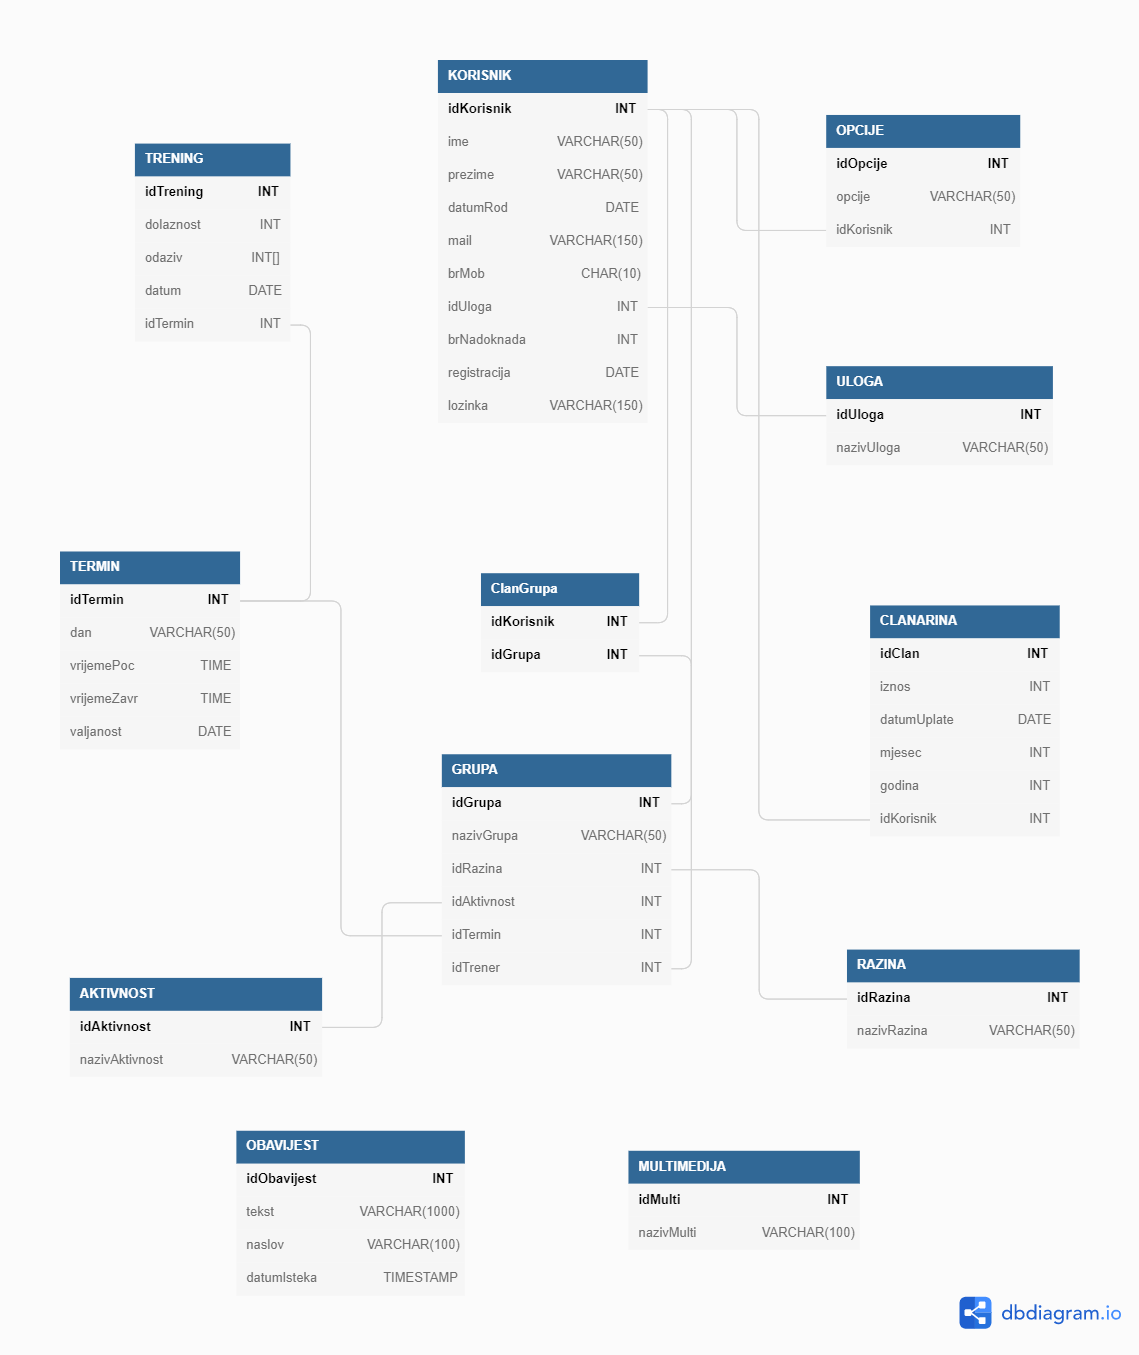
\includegraphics[scale=0.4]{slike/dijagram_baze.png}
            			\centering
            			\caption{Dijagram baze}
            			\label{fig:promjene}
            		\end{figure}
    			\eject
			
	\section{Aplikacija}
    	\noindent{Kada je aplikacija gotova, možemo provesti i završno ispitivanje. Svi testovi su provedeni ručno. Ispitivanje se izvodilo pa definiranim obrascima uporabe kako bi se što bolje pokrila funkcionalnost sustava. Također je i ispitano uobičajenim korištenjem kako bi se prouzročili "bugovi" s kojima bi se korisnik u svom korištenju mogao susrest. Ispitani su svi dijelovi sustava, no zbog jednostavnosti dokumentacije i nepotrebnog ponavljanja prikazani su samo neki. U prikazu se nalaze ispitivanja UC1, UC5, UC7, UC10, UC13, UC14, UC15, UC23, UC28}
			
		\noindent \textbf{Ispitni slučaj 1: Registracija korisnika}\\
			\textbf{Ulaz:}\\
			    \indent1. Pokretanje aplikacije.\\
			    \indent2. Upisivanje podataka potrebnih za registraciju.\\
			    \indent3. Pritisak na gumb "Dalje...".\\
			   
			\noindent\textbf{Očekivani rezultat:}\\
			    \indent1. Provjera validacije svih podataka.\\
			    \indent2. Preusmjerenje na stranicu za izbor Opcija i uspješna registracija.\\
			    
			\noindent\textbf{Rezultat:}
			    \noindent Očekivani rezultat je zadovoljen, korisnik je prijavljen i vraćen na početnu stranicu.
			    
			\begin{figure}[H]
        			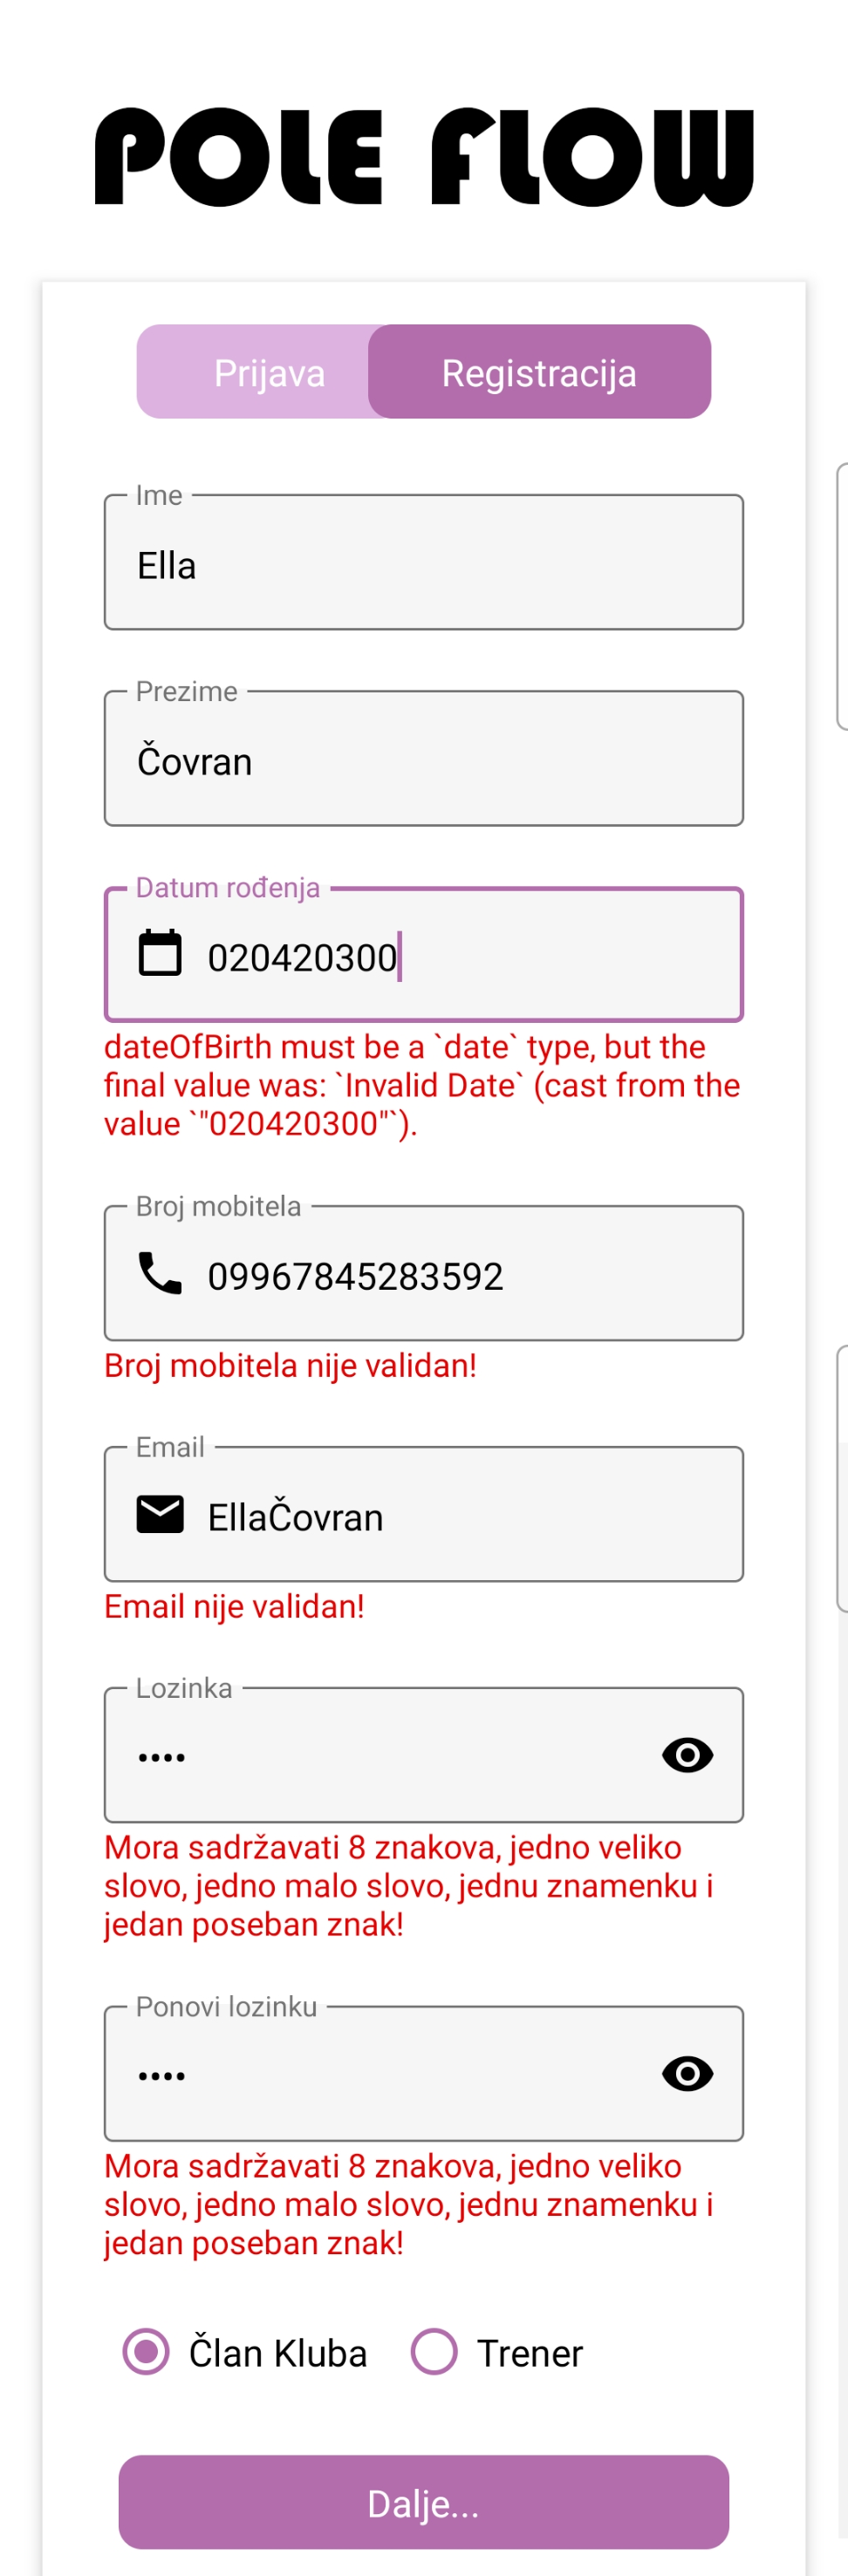
\includegraphics[scale=0.2]{slike/App_registracija.jpg}
        			\centering
        			\caption{Slika stranice za registraciju}
        			\label{fig:promjene}
        		\end{figure}
			    
	    \noindent \textbf{Ispitni slučaj 2: Pregled novoregistriranih korisnika}\\
			\textbf{Ulaz:}\\
			    \indent1. Pokretanje aplikacije.\\
			    \indent2. Prijava kao Administrator.\\
			    \indent3. Otvaranje početne stranice.\\
			   
			\noindent\textbf{Očekivani rezultat:}\\
			    \indent1. Prikaz svih korisnika, i njihovih opcija, koji su se registrirali od zadnjeg dana prijave administratora\\
			    
			\noindent\textbf{Rezultat:}
			    \noindent Očekivani rezultat je zadovoljen, korisniku se prikazuju informacije o novoregistriranim korisnicima.
			    
			\begin{figure}[H]
        			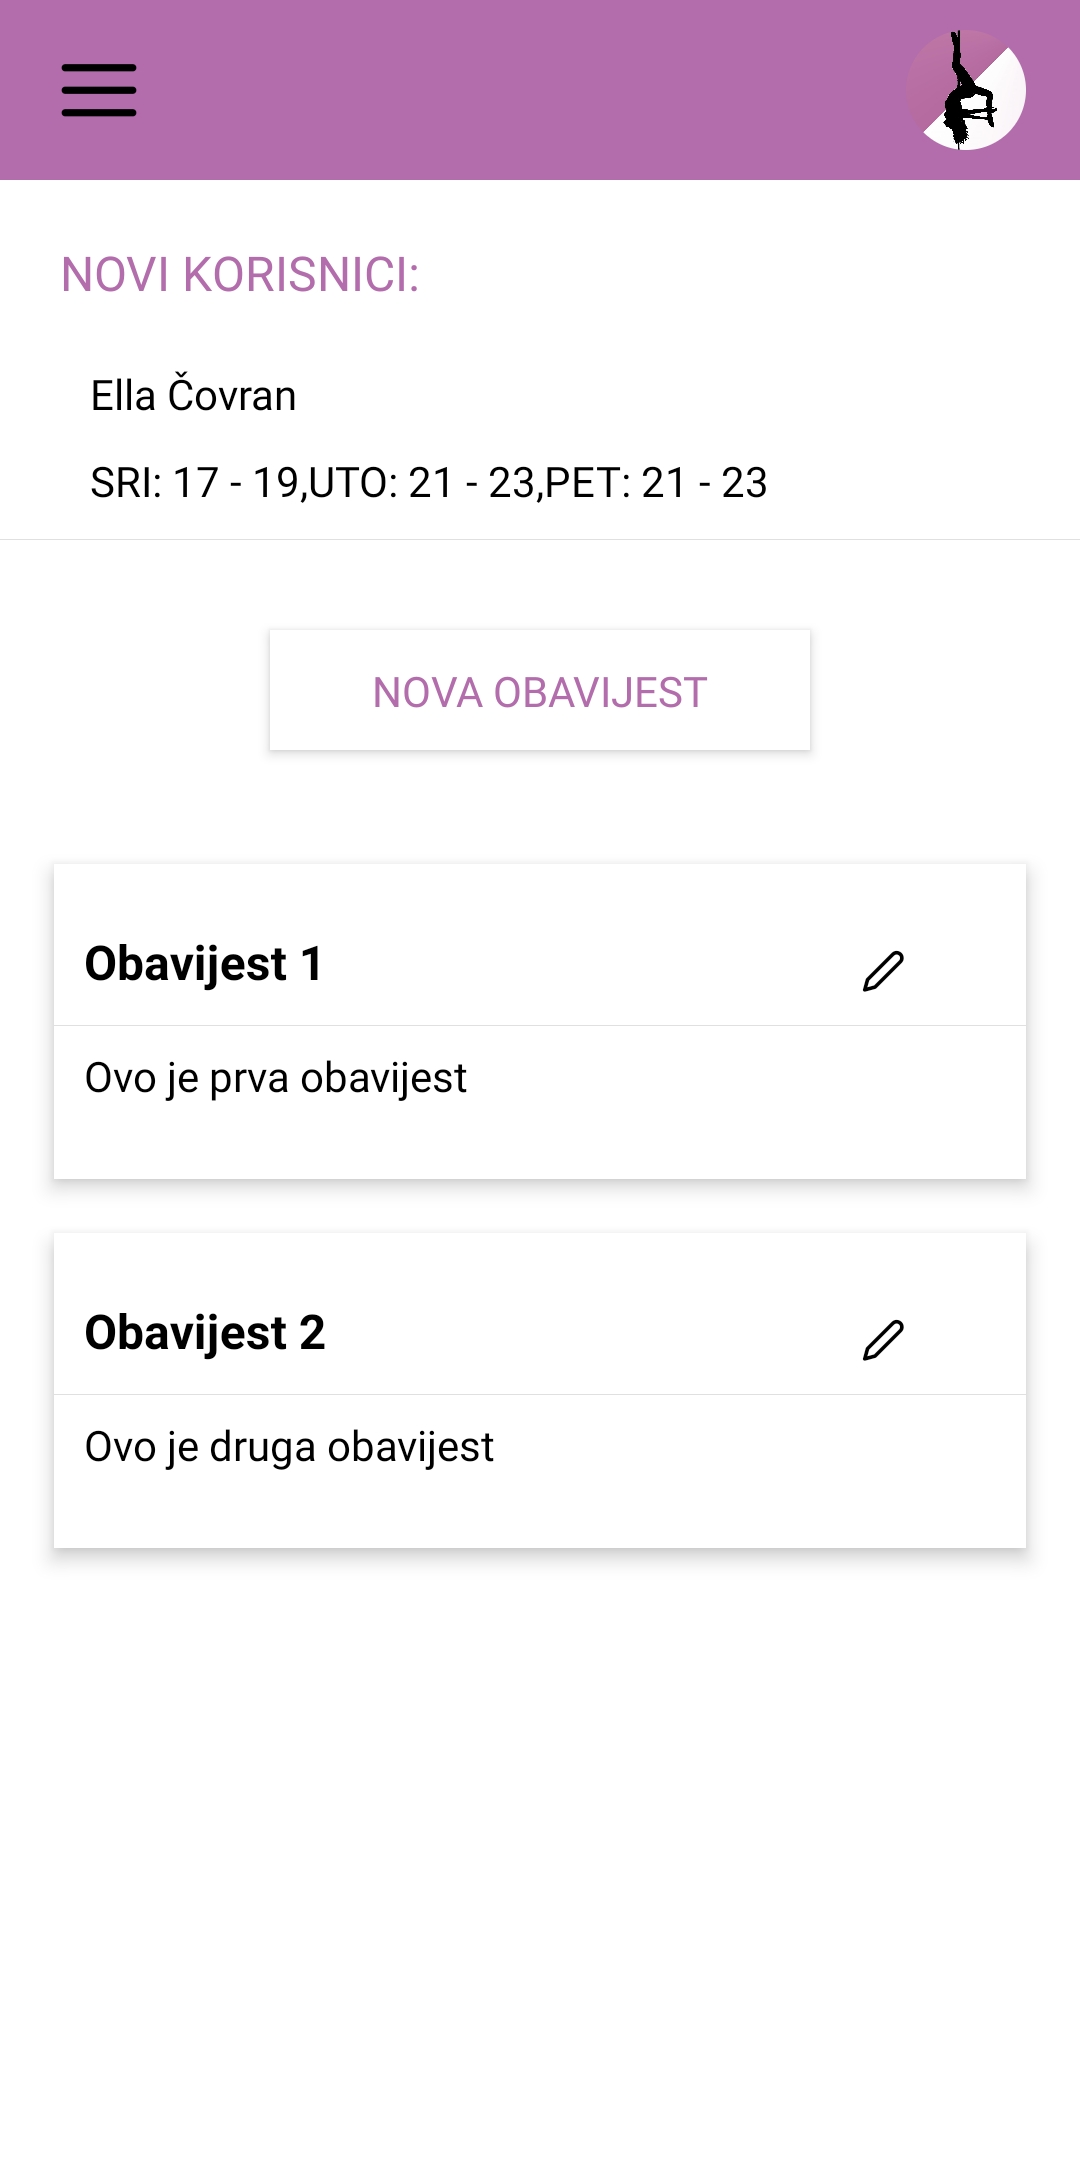
\includegraphics[scale=0.2]{slike/App_novi_korisnici_i_obavijesti.jpg}
        			\centering
        			\caption{Slika početne stranice sa popisom novoregistriranih korisnika}
        			\label{fig:promjene}
        		\end{figure}
        		
	    \noindent \textbf{Ispitni slučaj 3: Pregled članarine}\\
			\textbf{Ulaz:}\\
			    \indent1. Pokretanje aplikacije.\\
			    \indent2. Prijava.\\
			    \indent3. Otvaranje korisničkog profila.\\
			   
			\noindent\textbf{Očekivani rezultat:}\\
			    \indent1. U kvadratu "Članarine" se ispisuje iznos i status članarine za tekući mjesec.\\
			    
			\noindent\textbf{Rezultat:}
			    \noindent Očekivani rezultat je zadovoljen, korisniku se prikazuje članarina za tekući mjesec.
			    
			\begin{figure}[H]
        			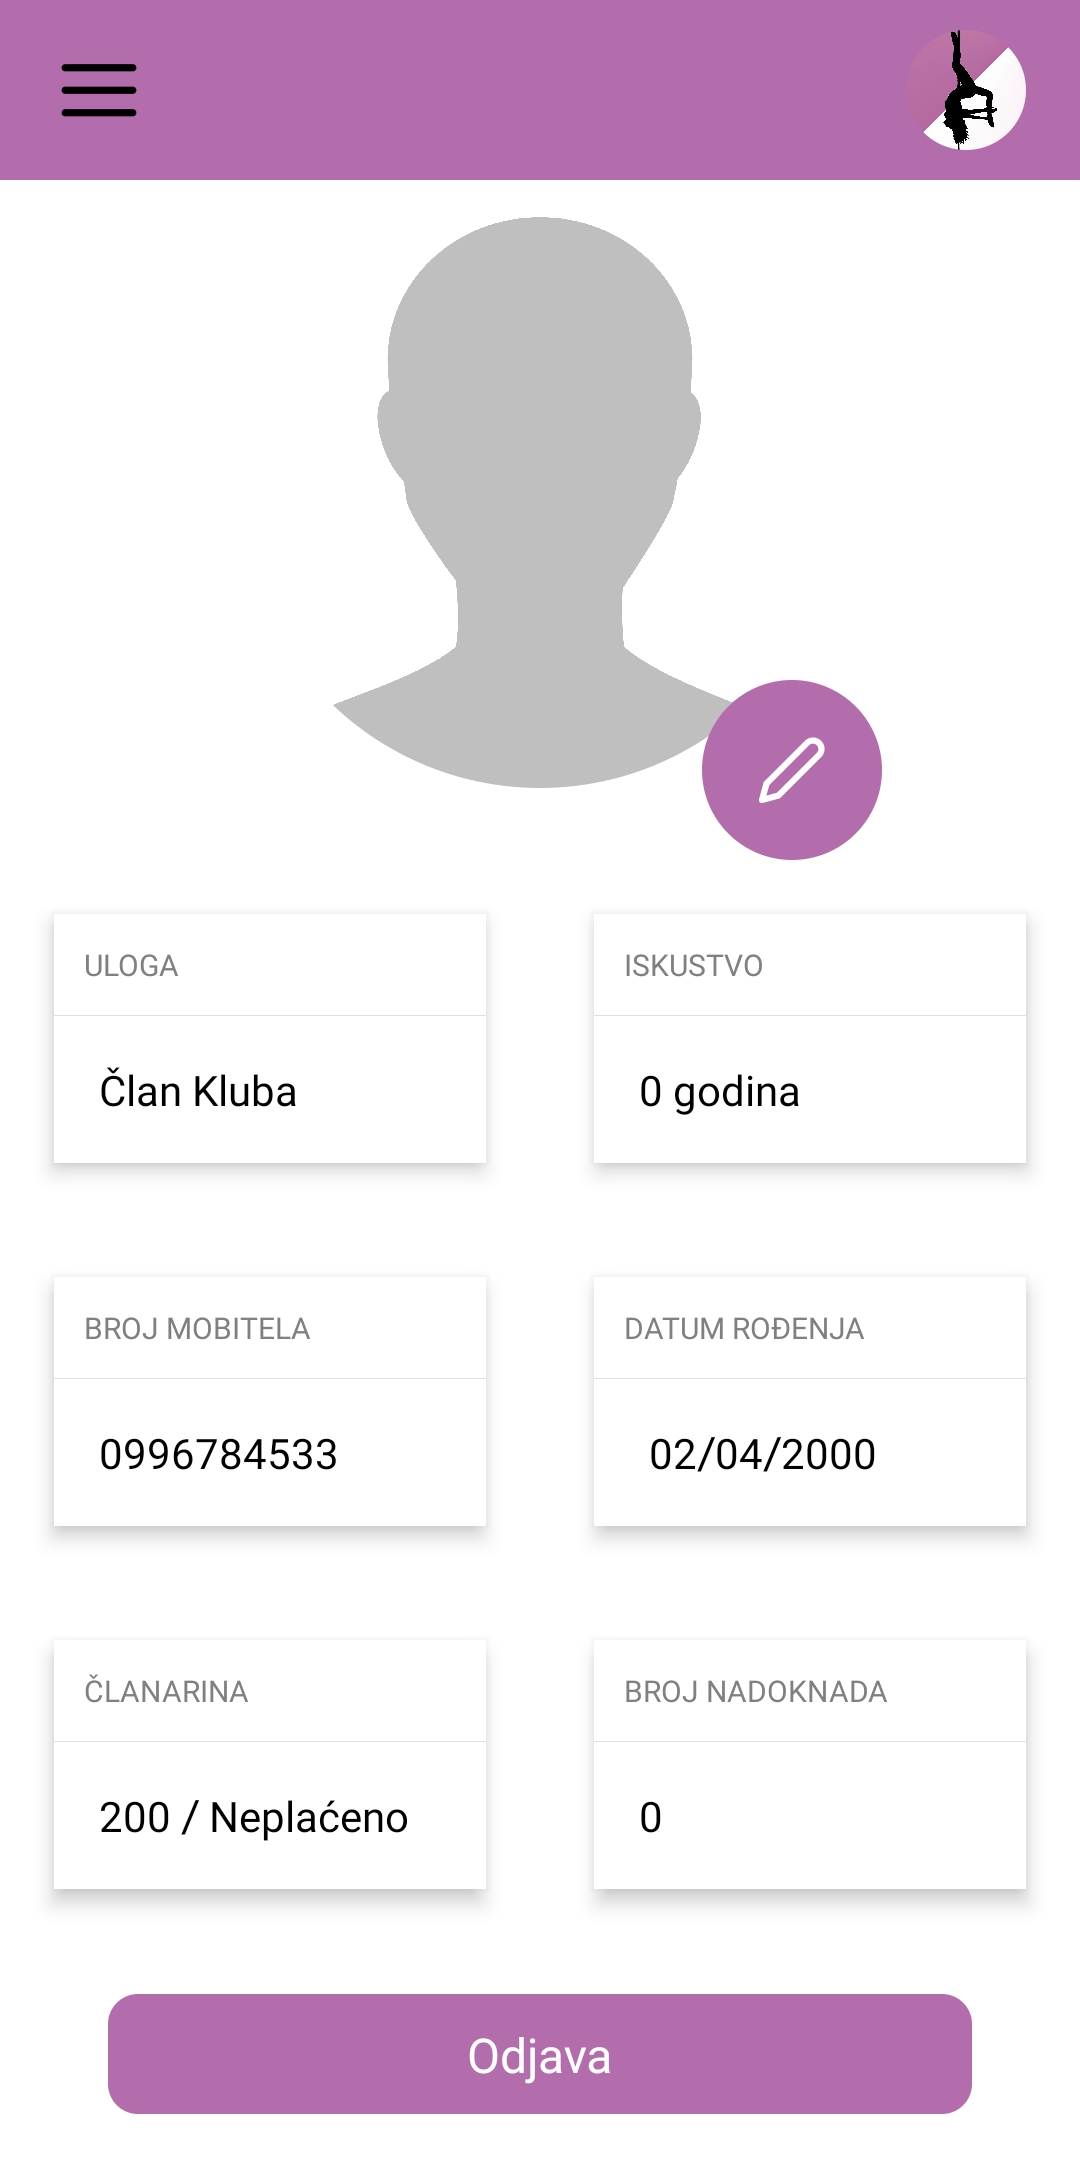
\includegraphics[scale=0.2]{slike/App_profil_neplaceno.jpg}
        			\centering
        			\caption{Slika stranice za korisnički profil}
        			\label{fig:promjene}
        		\end{figure}
        		
        \noindent \textbf{Ispitni slučaj 4: Uređivanje članarine korisnika}\\
			\textbf{Ulaz:}\\
			    \indent1. Pokretanje aplikacije.\\
			    \indent2. Prijava kao Administrator.\\
			    \indent3. Otvaranje stranice sa svim korisnicima.\\
			    \indent4. Odabir korisnika.\\
			    \indent5. Prikaz stanja prve 3 ne plaćene članarine. (poredane po datumima)\\
			    \indent6. Odabir "kvačice" uz članarinu koja je plaćena.\\
			   
			\noindent\textbf{Očekivani rezultat:}\\
			    \indent1. Pohrana podataka članarini i preusmjeravanje na stranicu sa svim korisnicima.\\
			    
			\noindent\textbf{Rezultat:}
			    \noindent Očekivani rezultat je zadovoljen, u bazu se pohranjuje datum uplate članarine te se korisnik preusmjerava na stranicu sa svim korisnicima.
			    
		    \begin{figure}[H]
        			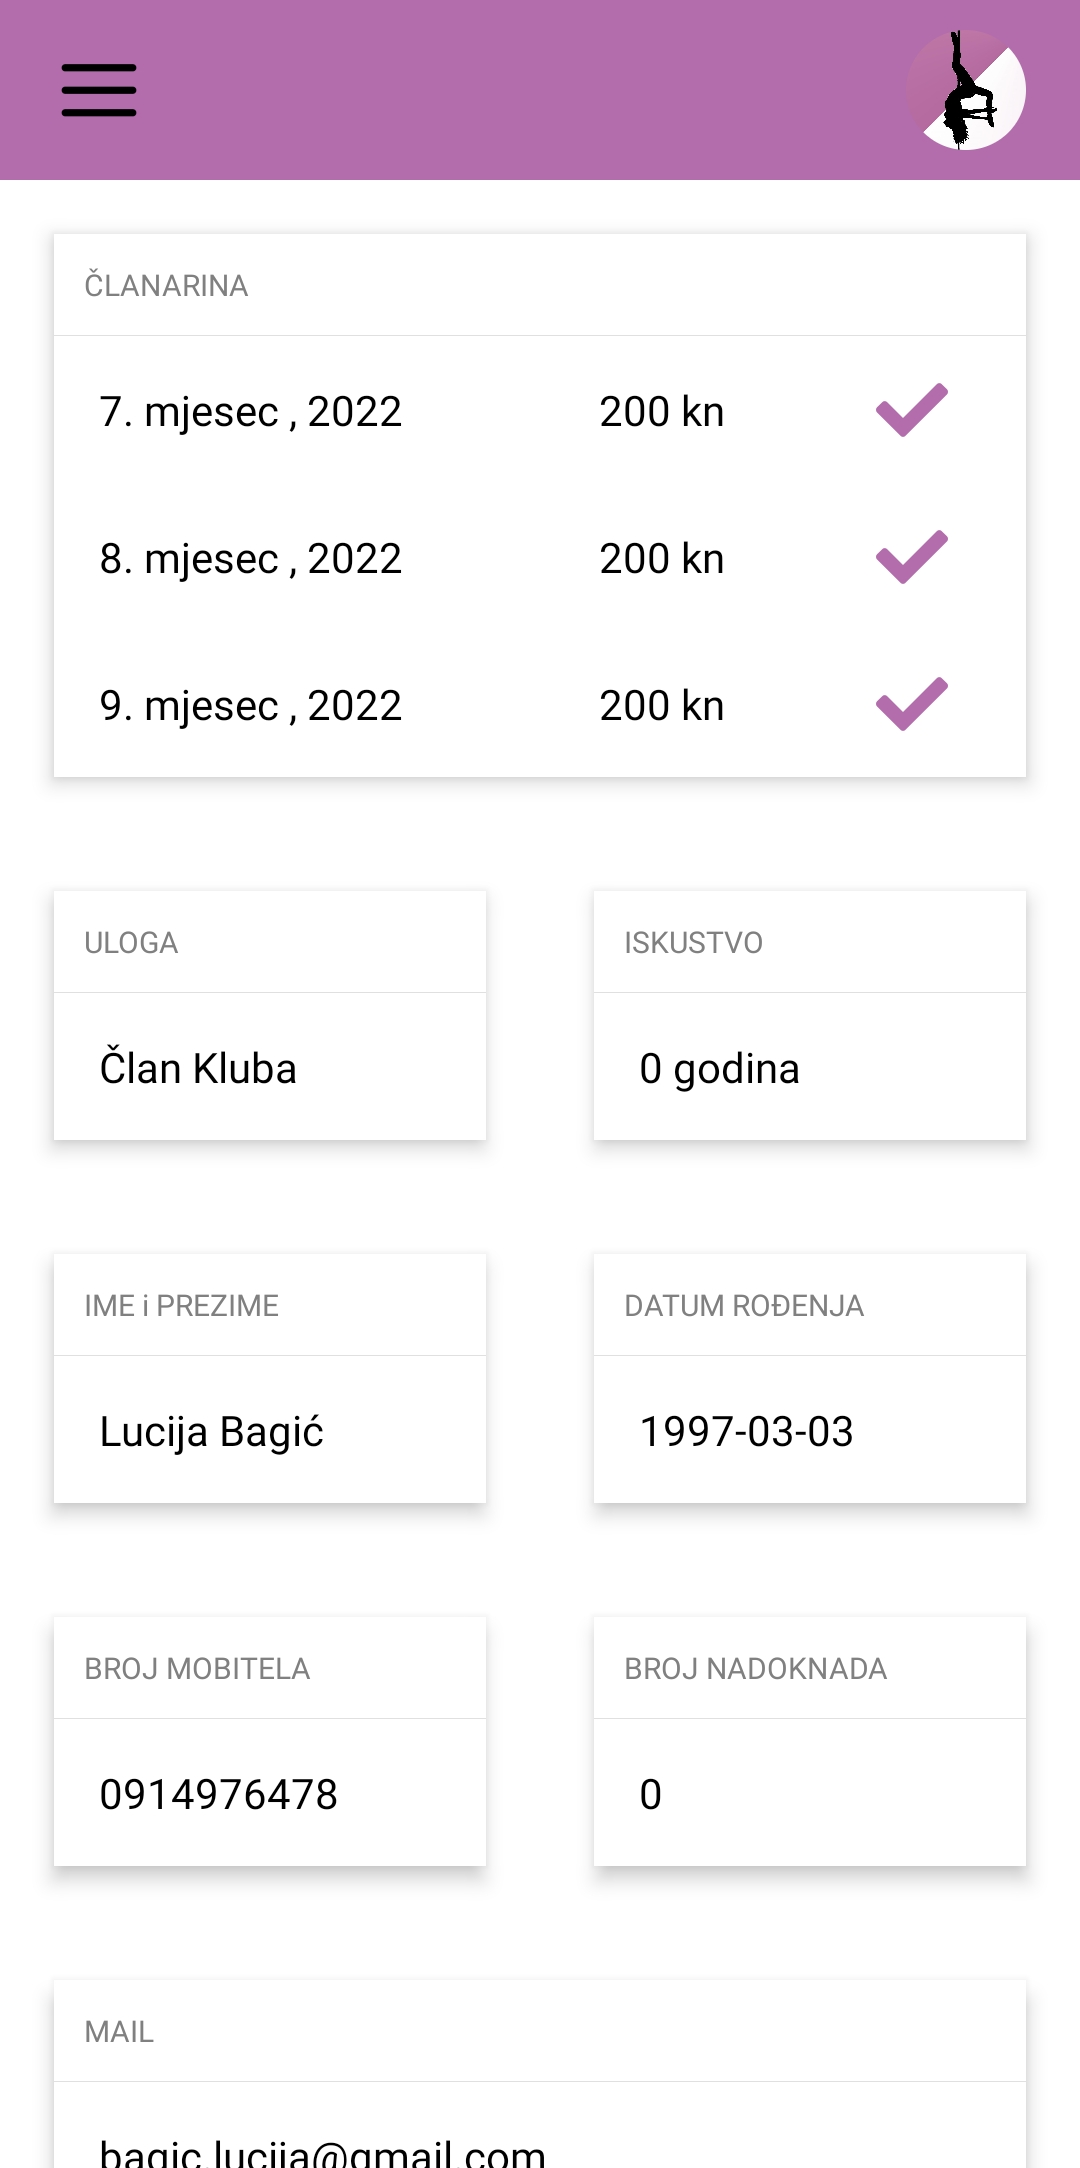
\includegraphics[scale=0.2]{slike/App_clanarine.jpg}
        			\centering
        			\caption{Slika stranice o korisniku}
        			\label{fig:promjene}
        		\end{figure}
			    
		\noindent \textbf{Ispitni slučaj 5: Pregled galerije}\\
			\textbf{Ulaz:}\\
			    \indent1. Pokretanje aplikacije.\\
			    \indent2. Prijava.\\
			    \indent3. Otvaranje galerije.\\
			    \indent4. Otvaranje određene fotografije iz galerije.\\
			   
			\noindent\textbf{Očekivani rezultat:}\\
			    \indent1. Prikaz svih fotografija iz galerije. Odabirom fotografije se otvara njena puna veličina.\\
			    
			\noindent\textbf{Rezultat:}
			    \noindent Očekivani rezultat je zadovoljen, korisniku se prikazuje fotografija te se može vratiti na stranicu galerije.
			    
			\begin{figure}[H]
        			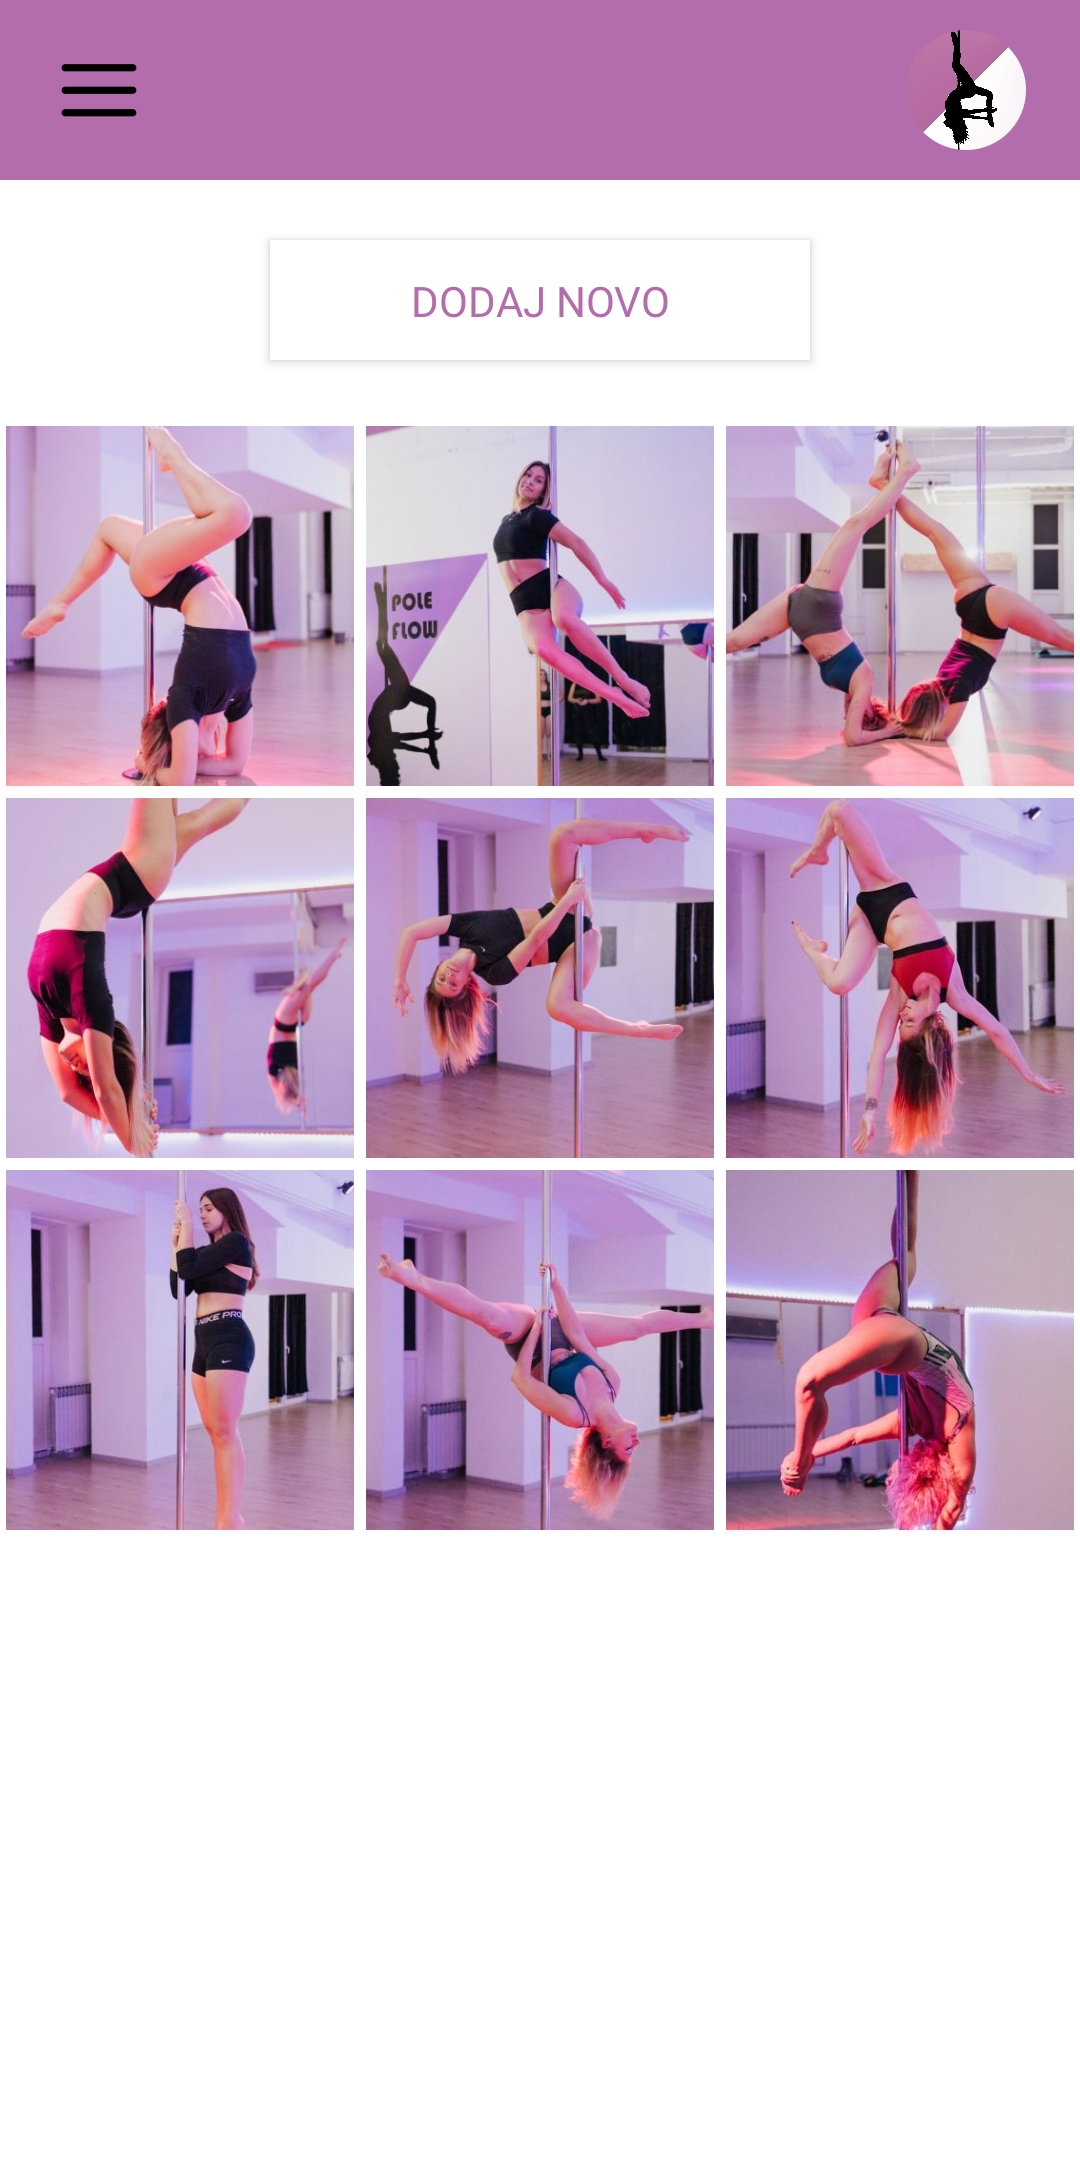
\includegraphics[scale=0.2]{slike/App_galerija.jpg}
        			\centering
        			\caption{Slika stranice galerije}
        			\label{fig:promjene}
        		\end{figure}
			    
		\noindent \textbf{Ispitni slučaj 6: Pregled rasporeda treninga}\\
			\textbf{Ulaz:}\\
			    \indent1. Pokretanje aplikacije.\\
			    \indent2. Prijava kao administrator.\\
			    \indent3. Otvaranje rasporeda treninga.\\
			   
			\noindent\textbf{Očekivani rezultat:}\\
			    \indent1. Prikaz svih treninga u kalendaru.\\
			    
			\noindent\textbf{Rezultat:}
			    \noindent Očekivani rezultat je zadovoljen, korisniku se prikazuju svi treninzi u kalendaru.
			    
			\begin{figure}[H]
        			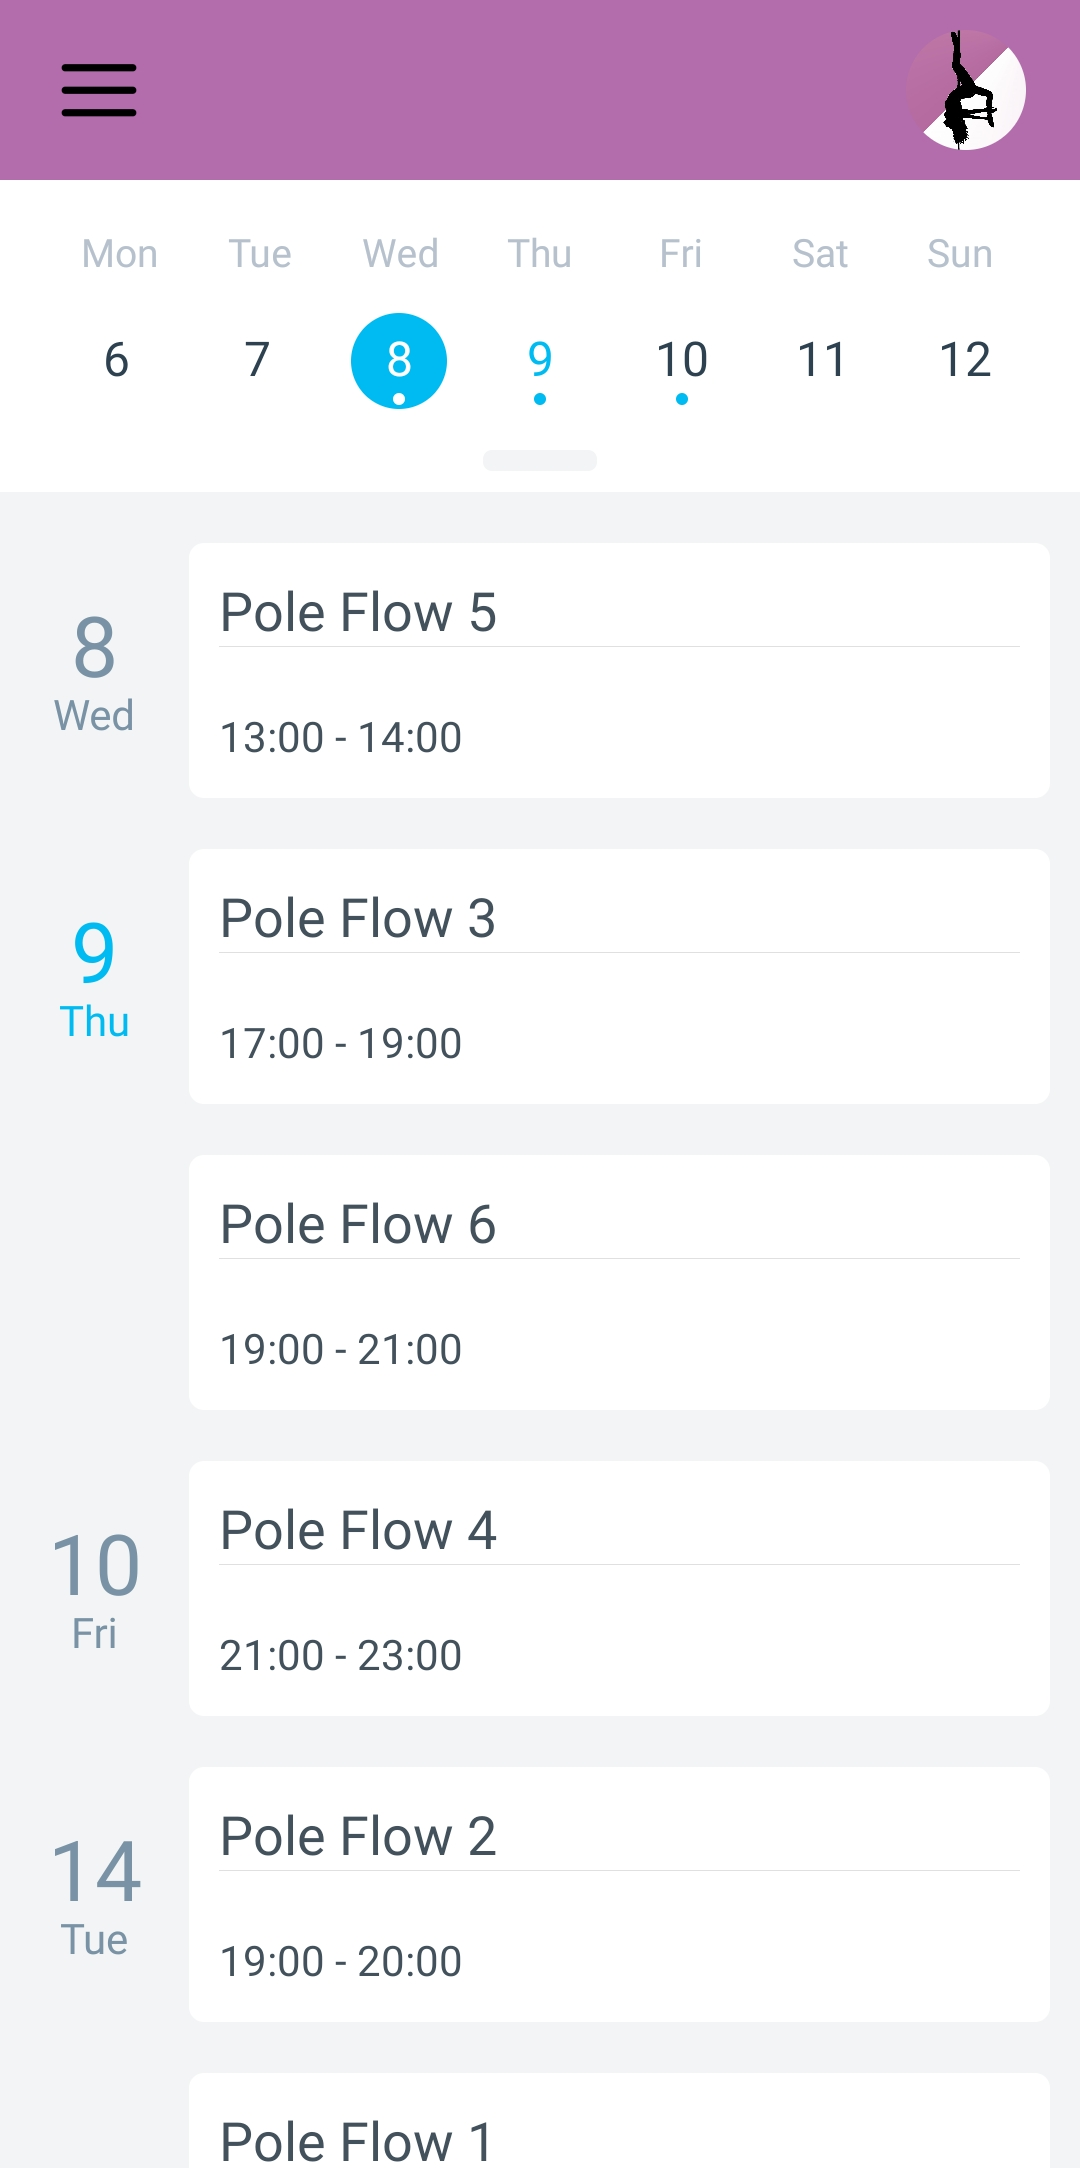
\includegraphics[scale=0.2]{slike/App_raspored_treninga.jpg}
        			\centering
        			\caption{Slika stranice za raspored treninga}
        			\label{fig:promjene}
        		\end{figure}
        		
		\noindent \textbf{Ispitni slučaj 7: Podsjetnik na trening}\\
			\textbf{Ulaz:}\\
			    \indent1. Pokretanje aplikacije.\\
			    \indent2. Prijava kao Član Kluba.\\
			    \indent3. Otvaranje početne stranice.\\
			    \indent4. Odabir "kvačice" u podsjetniku za "dolazak" na trening.\\
			   
			\noindent\textbf{Očekivani rezultat:}\\
			    \indent1. Prikaz podsjetnika na trening koji bi set trebao održati tog dana.\\
			    \indent1. Ažuriranje baze po pitanju odaziva na trening.\\
			    
			\noindent\textbf{Rezultat:}
			    \noindent Očekivani rezultat je zadovoljen, korisnikov dolazak se zabilježio u bazu ("odaziv" u tablici Trening).
			    
			\begin{figure}[H]
        			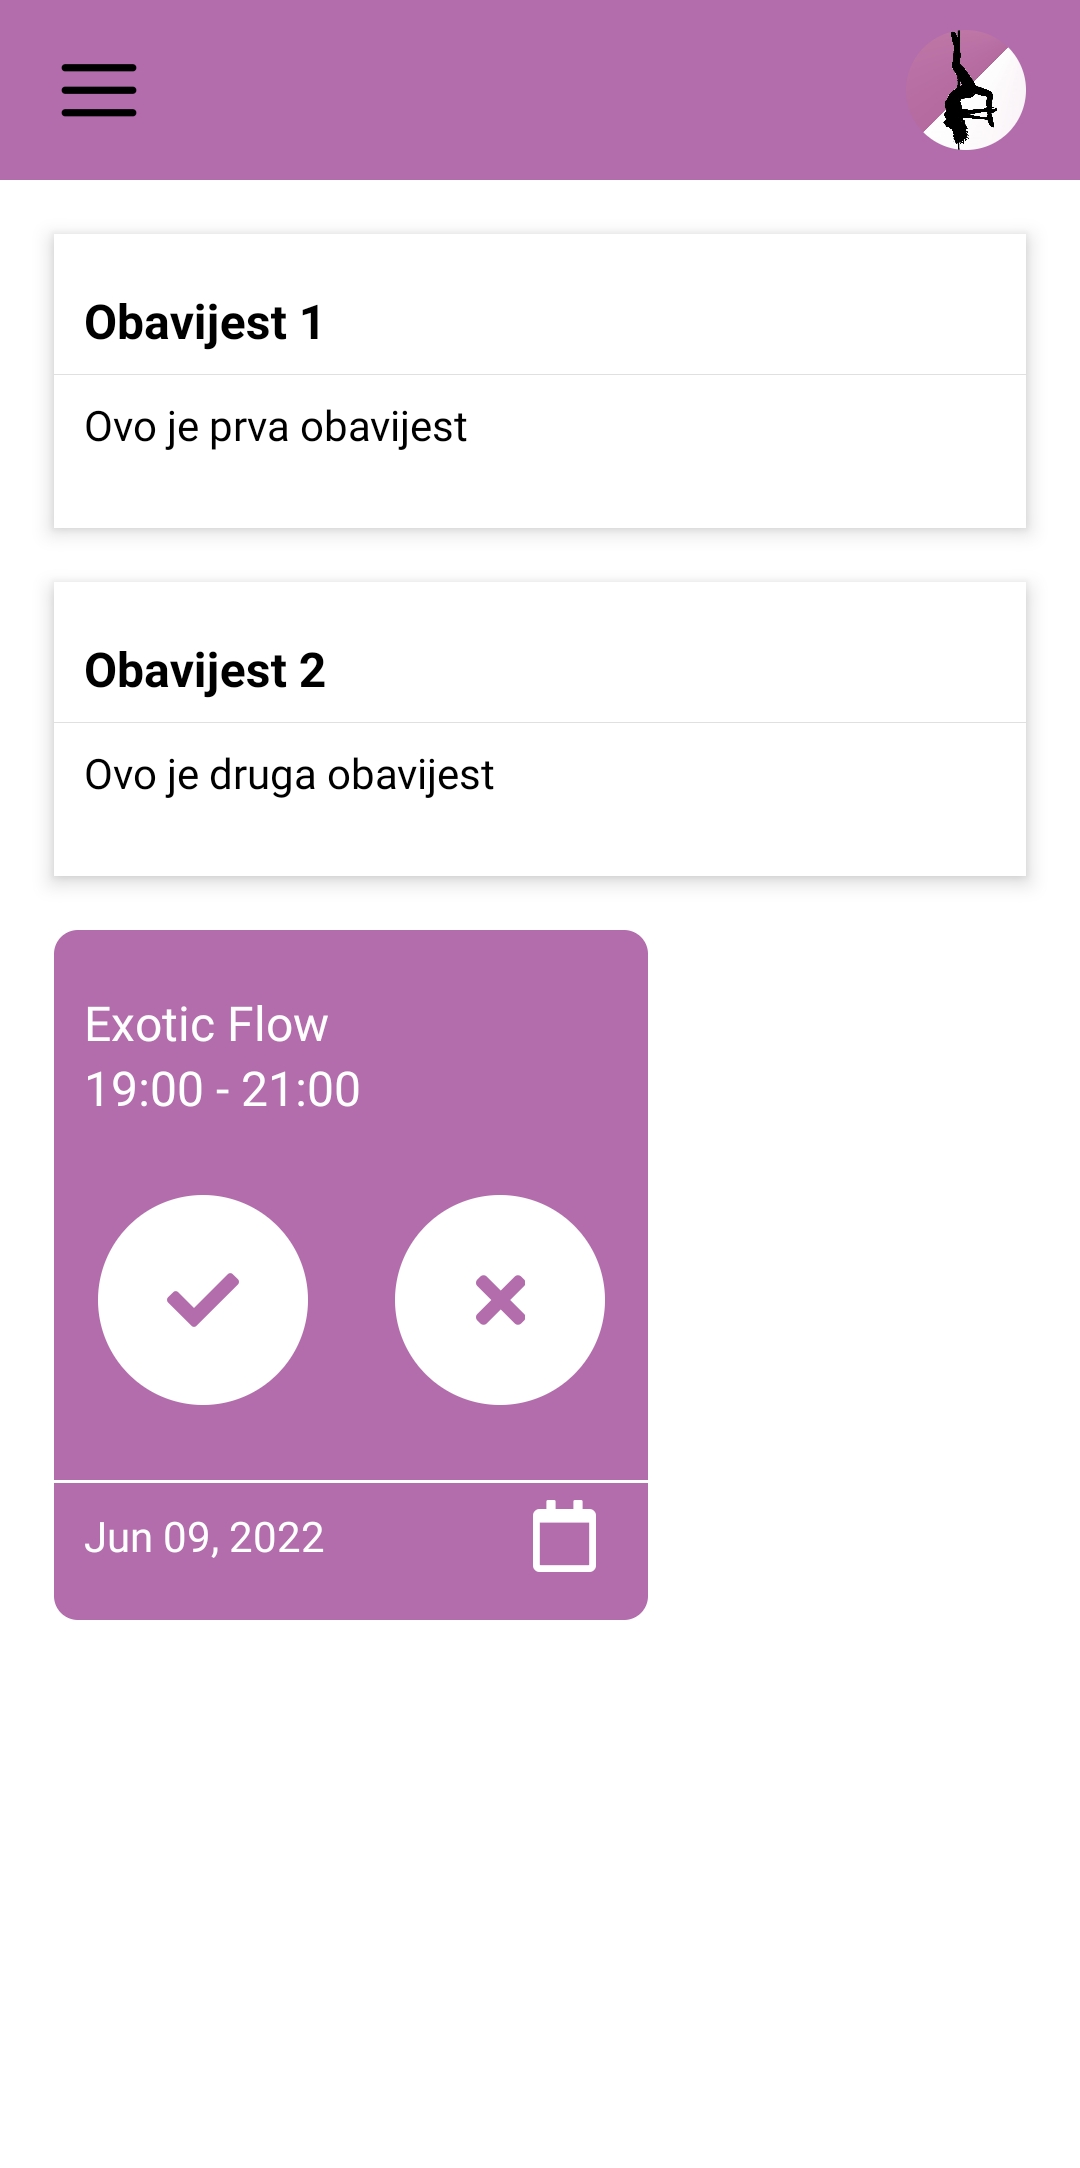
\includegraphics[scale=0.2]{slike/App_podsjetnik.jpg}
        			\centering
        			\caption{Slika početne stranice}
        			\label{fig:promjene}
        		\end{figure}
			    
	    \noindent \textbf{Ispitni slučaj 8: Informacije o nadolazećem treningu}\\
			\textbf{Ulaz:}\\
			    \indent1. Pokretanje aplikacije.\\
			    \indent2. Prijava kao Administrator.\\
			    \indent3. Otvaranje rasporeda treninga.\\
			    \indent4. Odabir treninga koji se nije još održao.\\
			   
			\noindent\textbf{Očekivani rezultat:}\\
			    \indent1. Prikaz informacija o nadolazećem treningu.\\
			    
			\noindent\textbf{Rezultat:}
			    \noindent Očekivani rezultat je zadovoljen, korisniku se prikazuju informacije o nadolazećem treningu.
			    
			\begin{figure}[H]
        			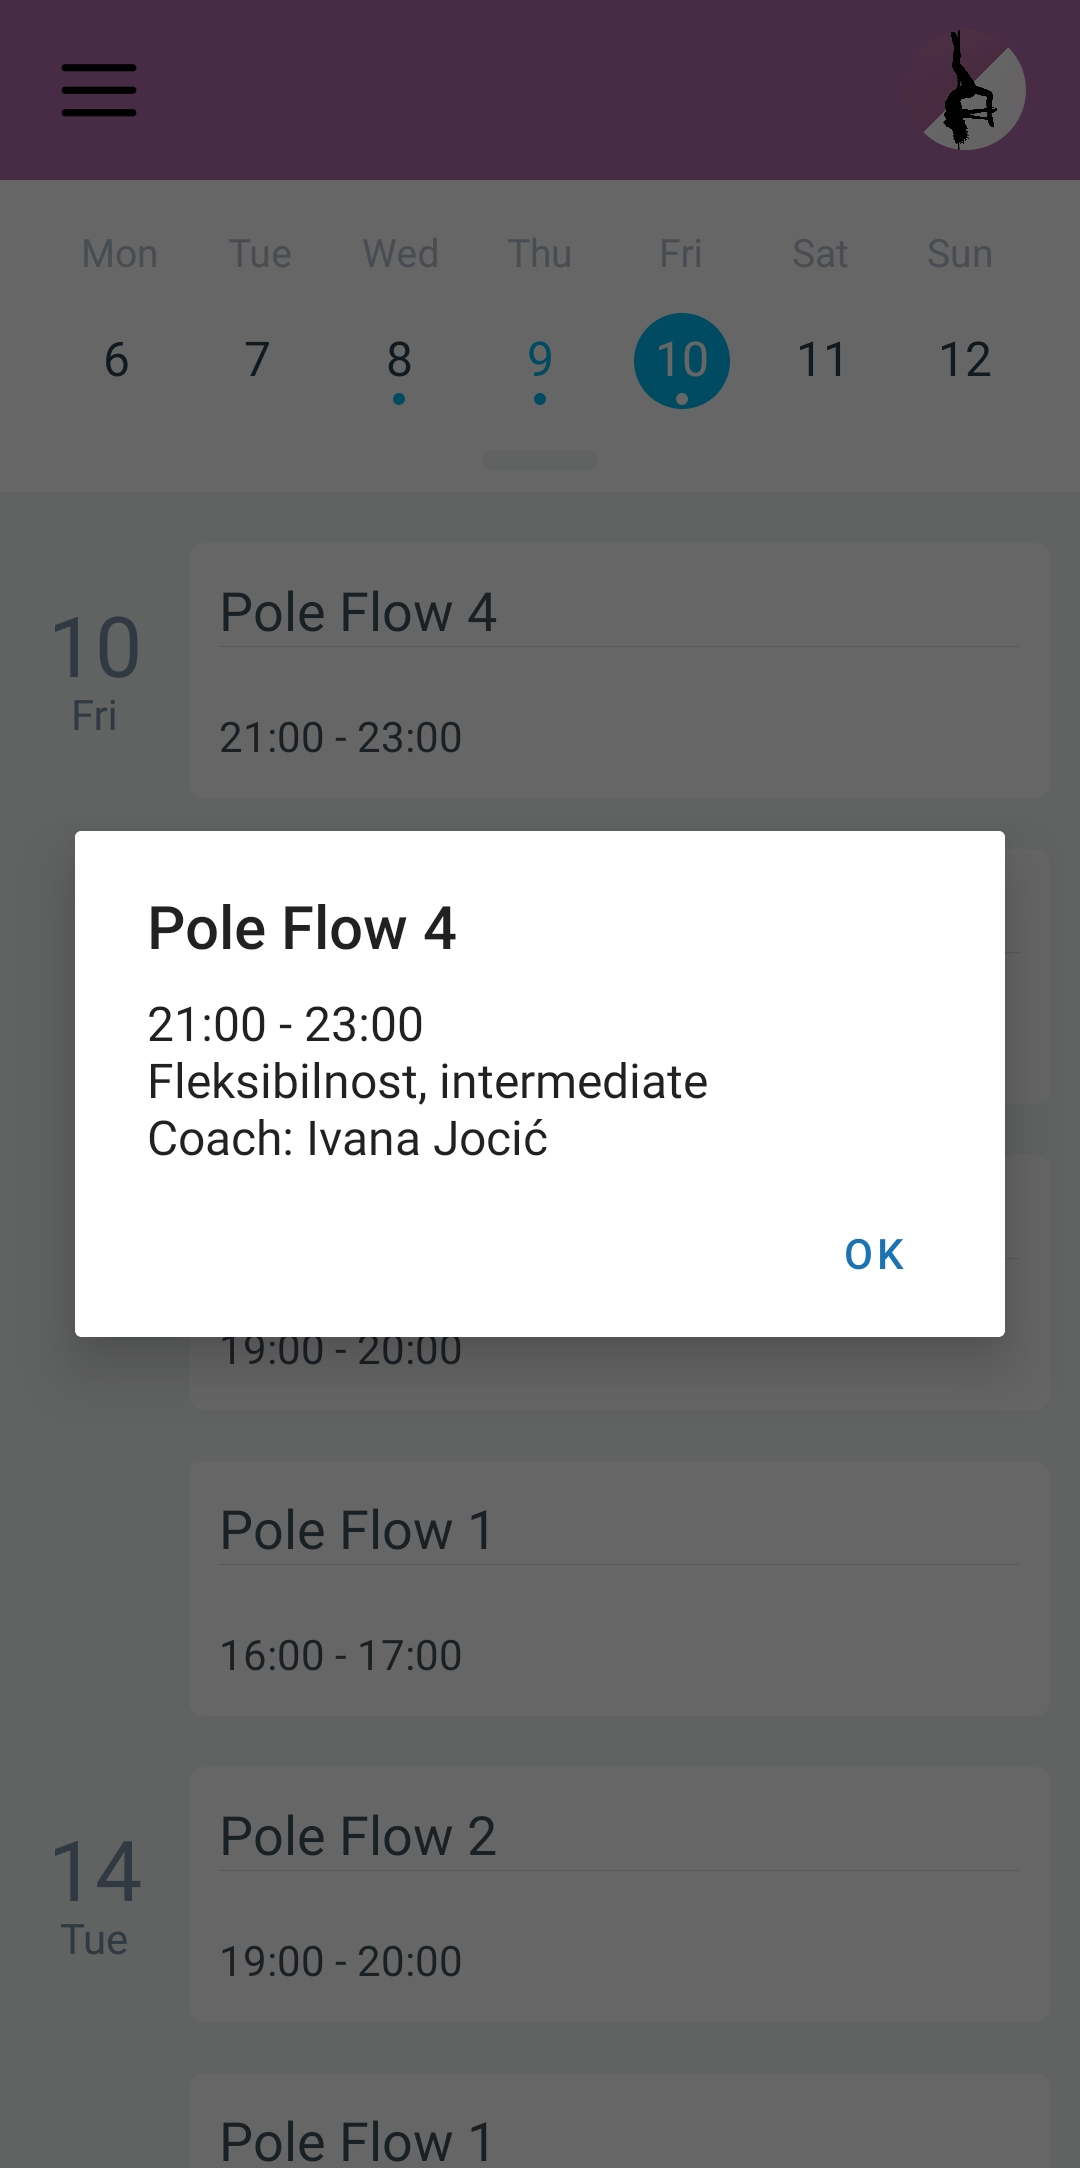
\includegraphics[scale=0.2]{slike/App_info_treninga.jpg}
        			\centering
        			\caption{Slika stranice za raspored treninga}
        			\label{fig:promjene}
        		\end{figure}
			    
		\noindent \textbf{Ispitni slučaj 9: Povratna informacija o dolaznosti na trening}\\
			\textbf{Ulaz:}\\
			    \indent1. Pokretanje aplikacije.\\
			    \indent2. Prijava kao Administrator.\\
			    \indent3. Otvaranje rasporeda treninga.\\
			    \indent4. Odabir treninga koji se održao.\\
			    \indent5. Odabir "kvačice" uz korisnika koji se pojavio, odnosno "križića" uz ono koji se nije pojavio na treningu.\\
			   
			\noindent\textbf{Očekivani rezultat:}\\
			    \indent1. Pohrana podataka o nadoknadama i dolaznosti na trening.\\
			    
			\noindent\textbf{Rezultat:}
			    \noindent Očekivani rezultat je zadovoljen, u bazu se pohranjuju novi brojevi nadoknada (tablica Korisnik) te dolaznost na trening (tablica Trening).
			    
			\begin{figure}[H]
        			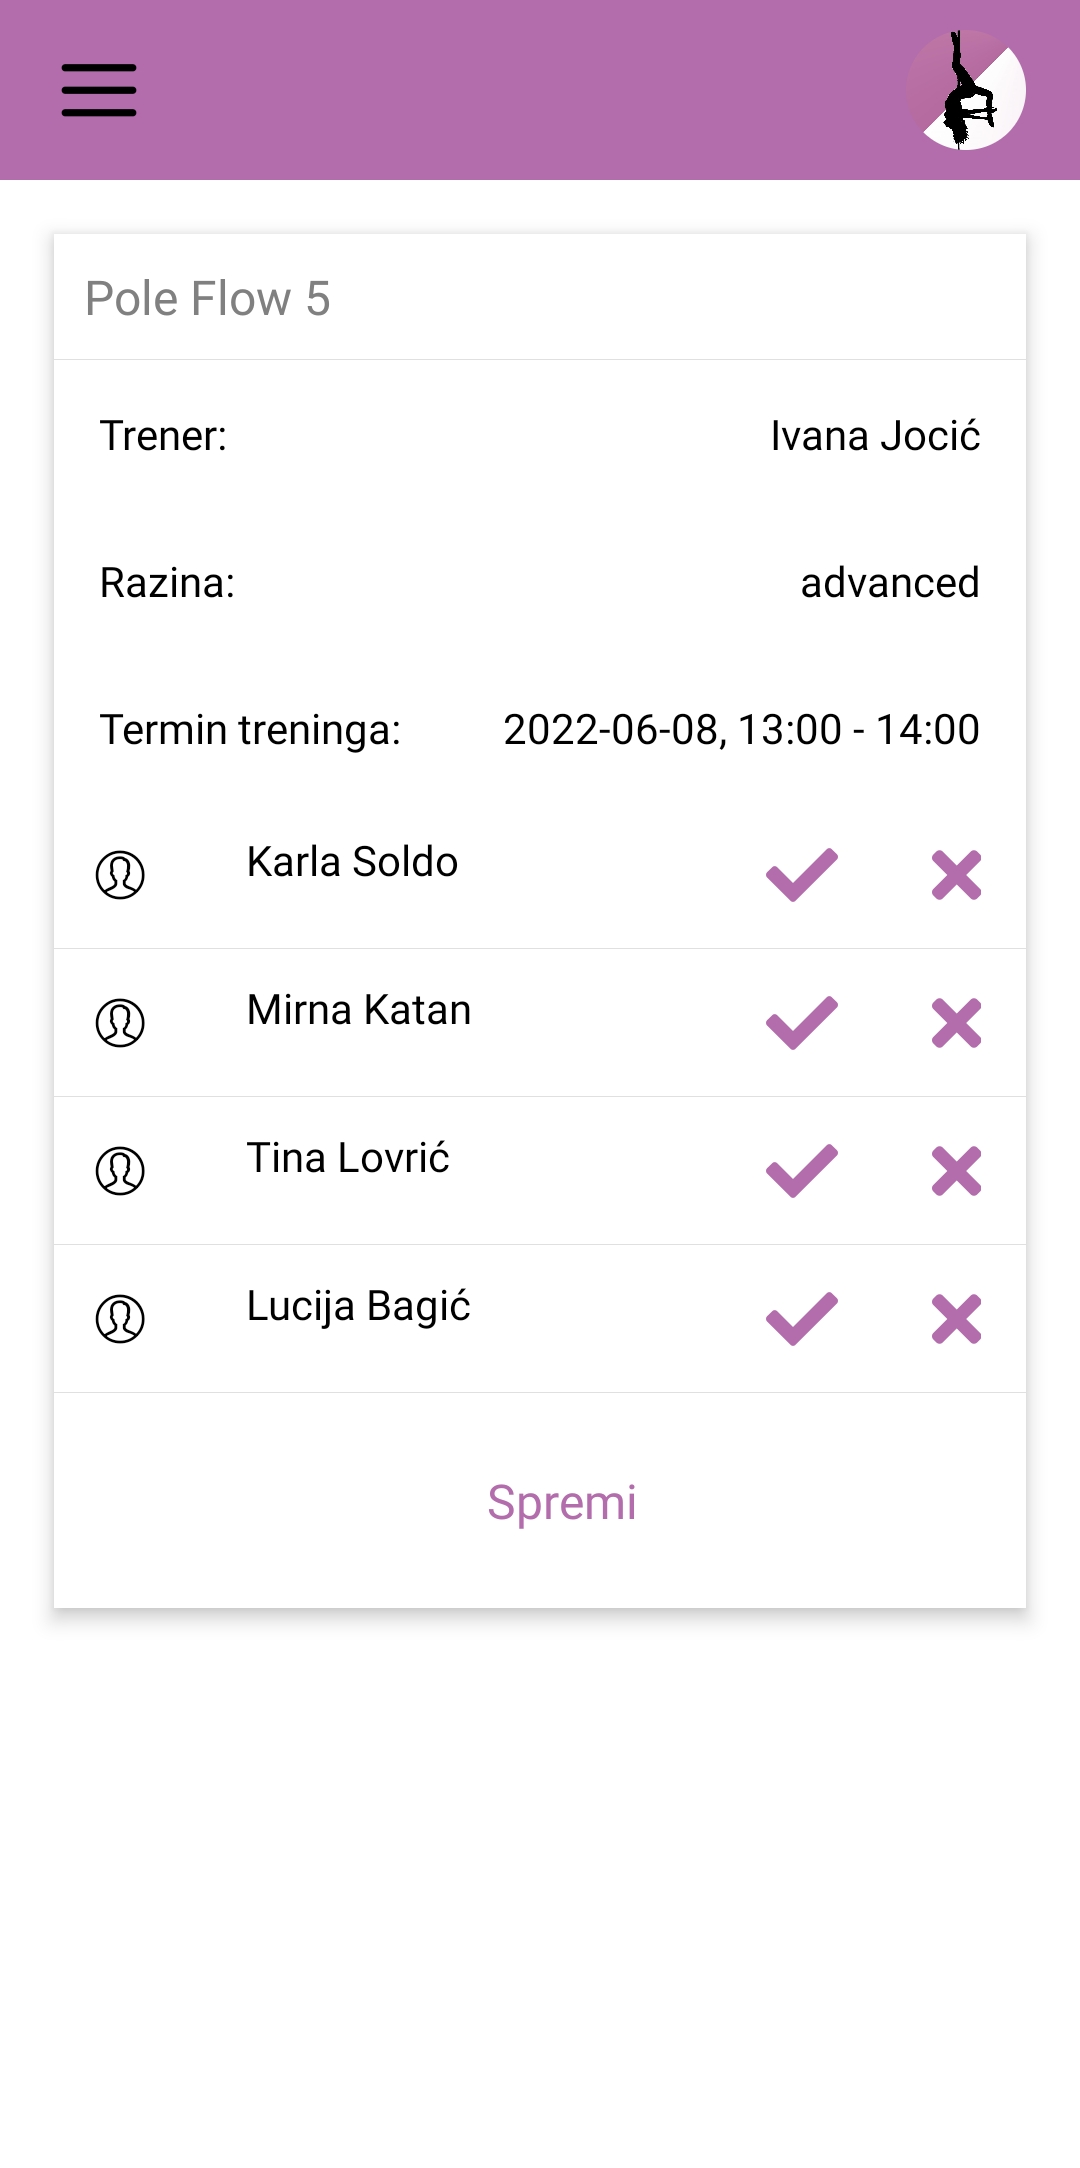
\includegraphics[scale=0.2]{slike/App_dolaznost.jpg}
        			\centering
        			\caption{Slika stranice za raspored treninga}
        			\label{fig:promjene}
        		\end{figure}
			    
			    
		

    \section{Upute za puštanje u pogon}
			 
			 
			 \textbf{Instalacija, konfiguracija i punjenje baze podataka}\\
			 \noindent Potrebno je preuzeti pgAdmin za operacijski sustav Windows i provesti preporučenu instalacija. Prilikom prvog pokretanja aplikacije potrebno je odrediti lozinku koja se upisuje pri paljenju. Nakon prijavljivanja potrebno je kreirati bazu podataka s nazivom \textit{poleflow}. Naziv mora biti isto napisan kao u tekstu, inače aplikacija neće radit. U stvorenoj bazi otvoriti "Query tool" i kopirati cijeli dokument baza.sql koji se nalazi u mapi ../server/utils.
			
			 Prije pokretanja aplikacija je potrebno instalirati na računalo \textit{Android Studio}\footnote{\url{https://developer.android.com/}} ili preuzeti na mobitel \textit{Expo aplikaciju}\footnote{\url{https://expo.dev/}} putem \textit{Google Play-a}\footnote{\url{https://play.google.com/store/apps/details?id=host.exp.exponent&hl=en&gl=US}}. Potrebno je podesiti IP adresu u ../mobile/api.js datoteci. Podešena IP adresa mora biti jednaka i na mobitelu i na laptopu u slučaju pokretanja putem Expo mobilne aplikacije. Pokretanje simulatora se ostvaruje skeniranje QR koda preko mobilne aplikacije ili povezivanje s Expo Developer Tools-ima preko Andorid Studija.
			
			
			\eject 
			
	\section{Korist i postojeća slična rješenja}
		Na tržištu se nalazi mnogo planera, aplikacija za organizaciju i rasporede,aplikacija za tjelovježbu itd. Pregledom rada više različitih mobilnih aplikacija sam stvorila ideju za \textit{Pole Flow App}. Aplikacija je napravljena specifično za plesni kluba, a ne za općenitu upotrebu, no manjim modifikacijama (aktivnosti, iznos članarina, uloge korisnik, ...) bi aplikacija funkcionirala i za druge sportske klubove. Cilj aplikacije je bio da se bolje organiziraju treninzi i komunikacija među korisnicima.
		
		\pagebreak

\chapter{Zaključak}
    Zadatak za završni rad bio je razvoj mobilne aplikacije za podršku aktivnostima plesnog kluba \textit{Pole Flow}. Aplikacija služi lakšoj organizaciji svih aktivnosti plesnog kluba. Nakon 15 tjedana razvoja ostvaren je zadani cilj. Provedba razvoja bila je podijeljena u tri faze.\\
    Prva faza projekta počinjala je izborom teme. Izbor je bio lagan s obzirom na to da sam znala da je plesnom klubu potrebna aplikacija zbog lakše organizacije i komunikacije. Konzultacijama s vlasnicom i glavnom trenericom kluba sam napisala početne zahtjeve aplikacije koji su se s vremenom pomalo mijenjali. S obzirom na ideju, odabir alata i jezika je također bio očit. Zbog lakoće rukovanja odlučila sam se za mobilnu aplikaciju. S obzirom na to da sam se u prošlom semestru susrela s React-om, nije bilo toliko teško prilagoditi se React Native-u.\\
    Druga faza projekta se poprilično razlikovala od prve i po trajanju i po načinu rada. Za razliku od prve faze, u drugoj je bio puno veći naglasak na implementaciji. Zbog manjka iskustva, morala sam samostalno učili nove alate i frameworke kako bi uspješnije implementirala rješenje. Započela sam s razvojem frontenda svih stranica zbog neiskustva u tom području. Frontend je rađen po skici izgleda razvijene u alatu Figma. Kada je baza frontenda bila dovršen sam započela povezivanje sa backend-om i bazom podataka.\\
    Treća faza projekta je bila testiranje, optimizacija te provjera projekta kao i pisanje dokumentacije. Tijekom ove faze sam uočila i neke nedostatke koje sam popravljala paralelno uz pisanje dokumentacije.\\
    Ovaj projekt je bio veoma vrijedno iskustvo jer sam se prvi put susrela radom mobilne aplikacije. Drago mi je što sam radila aplikaciju za plesni klub u kojem osobno treniram jer sam imala uvid u potrebe aplikacije. Tijekom razvoja sam se konzultirala sa svojom trenericom i vlasnicom kluba kako bih znala u kojem smjeru razvijati aplikaciju. Programski sustav se uvijek treba razvijati i obnavljati, uvijek se može poboljšati sigurnost te optimizirati sustav, no zadovoljna sam s postignutim rezultatom s obzirom na dobiveno vrijeme i znanje.
    
     

\bibliography{literatura}
		
		\begin{enumerate}
			
			
			\item  Programsko inženjerstvo, FER ZEMRIS, \url{http://www.fer.hr/predmet/proinz}
			
			\item  dbdiagram.io, \url{https://dbdiagram.io/}
			
			\item  React Native, \url{https://reactnative.dev/}
			
			\item  PostgreSQL, \url{https://www.postgresql.org/}
			
			\item  W3Schools, \url{https://www.w3schools.com/}
			
			\item  React Native Calendars, \url{https://wix.github.io/react-native-calendars/}
			
			\item  React Native Paper, \url{https://callstack.github.io/react-native-paper/}
			
			\item Figma, \url{https://www.figma.com/}
			
		\end{enumerate}
\bibliographystyle{fer}

\begin{sazetak}
Pole Flow App je mobilna aplikacija za plesni klub Pole Flow. Za frontend je uz to korišten alat React Native, a za backend je korišten programski okvir Express. Aplikacija će služiti za lakšu organizaciju treninga i članova kluba. Cilj aplikacije je riješiti sve probleme koji se javljaju pri organizaciji i komunikaciji pomoću jedne mobilne aplikacije. Novi članovi i treneri će pri učlanjenju u klub dobiti pristup aplikaciji te se registrirati u sustav. Imat će mogućnost uvida u raspored treninga, galeriju, korisničke podatke te obavijesti vezanih za klub. Članovi kluba imaju obavezu davanja povratne informacije o dolasku ili nedolasku na nadolazeći trening. Preko aplikacije, također se može pratiti broj nadoknada treninga te stanje članarine. Za sva uređivanja, dodavanja i brisanja je zaslužan administrator. 

\kljucnerijeci{mobilna aplikacija, organizacija, React Native, Express, plesni klub,raspored, galerija.}
\end{sazetak}

% TODO: Navedite naslov na engleskom jeziku.
\engtitle{Pole Flow App}
\begin{abstract}
The Pole Flow App is a mobile app for the Pole Flow dance club. For the frontend, the React Native tool and for the backend, the Express program framework was used. The application will serve to facilitate the organization of coaches and club members. The goal of the application is to solve all the problems that occur during organization and communication using one mobile application. New members and coaches will gain access to the application and register in the system when joining the club. They will have the opportunity to see the training schedule, gallery, user data and information related to the club. Club members have an obligation to give feedback on arrival or non-arrival at the upcoming training. Through the application, you can also monitor the number of training compensations and the status of membership fees. The administrator is responsible for all edits, additions and deletions.

\keywords{mobile app, organization, React Native, Express, dance club, schedule, gallery.}
\end{abstract}

\end{document}
